\subsection{Results}
The purpose of this section is to compare some of the different methods mentioned in the previous section \nameref{section:registration_previous_work}. Each of these methods produces a different transformation matrix. They are all applied on the point clouds created from the ChArUco board corners, see figure \ref{figure:pc_arucoboard}. It is supposed that a perfect transformation matrix should align exactly both point clouds. The mean absolute error is calculated for each point to estimate the error of each method. The steps for all experiments are the following:

\begin{enumerate}
    \item Estimate the rigid transformation matrix
    \item Transform one view into the other one with the estimated transformation matrix
    \item Calculate the mean absolute error (MAE) between the matching points of the ChArUco board of both views in each direction. The definition of the coordinates was presented in section \ref{section:3D coordinate system}.
\end{enumerate}

\subsubsection{Global registration}
\label{section:Global registration result}
\textbf{Experiment 1}

In this experiment, the procedure presented in section \ref{section:Global registration} is applied. A selected frame of the static scene is chosen. The two point clouds of the two different views are created. Without any transformation, the scene looks like in figure \ref{figure:pc_raw_static_merged}

\begin{figure}[H]
\centering
  \begin{subfigure}[b]{0.48 \textwidth}
    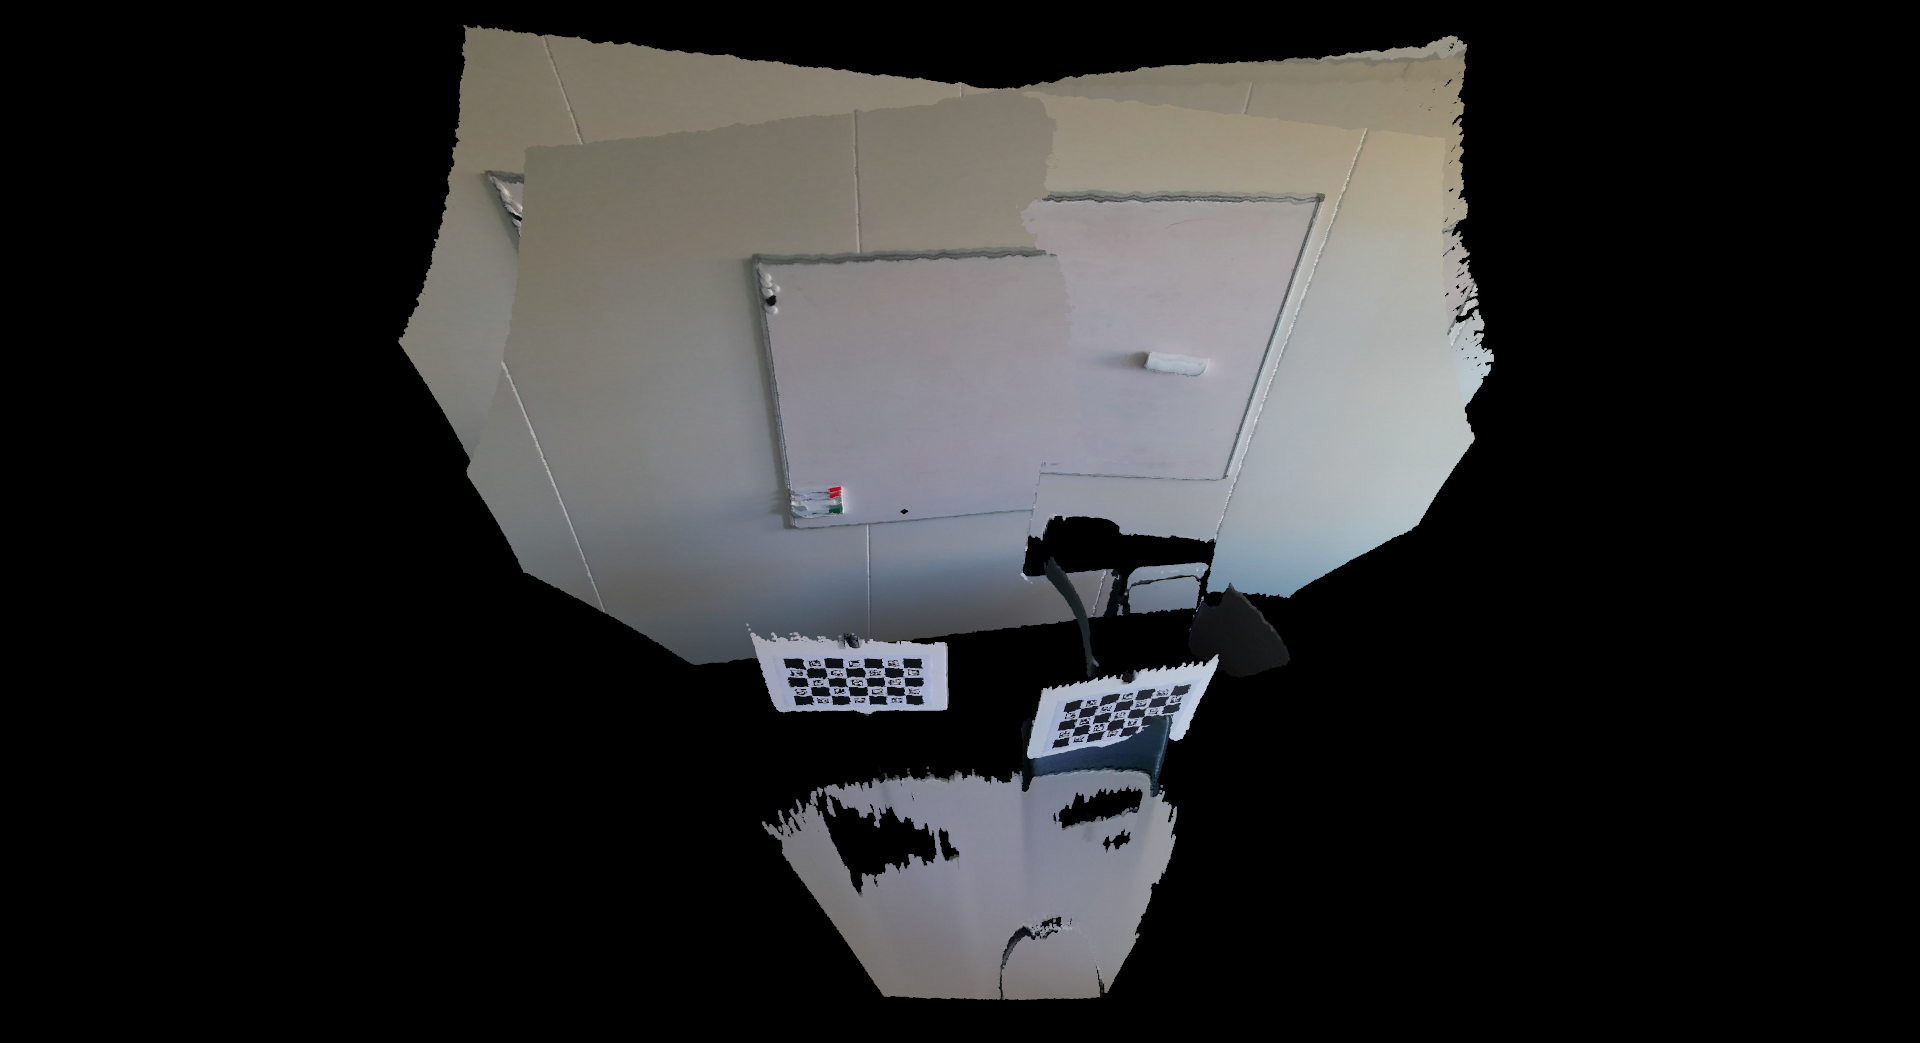
\includegraphics[width=\textwidth]{images/registration/pc_raw_static_merged_rgb.png}
    \caption{Merge of the two point clouds in RGB}
    \label{figure:pc_raw_static_merged_rgb}
  \end{subfigure}
  \hfill
  \begin{subfigure}[b]{0.48 \textwidth}
    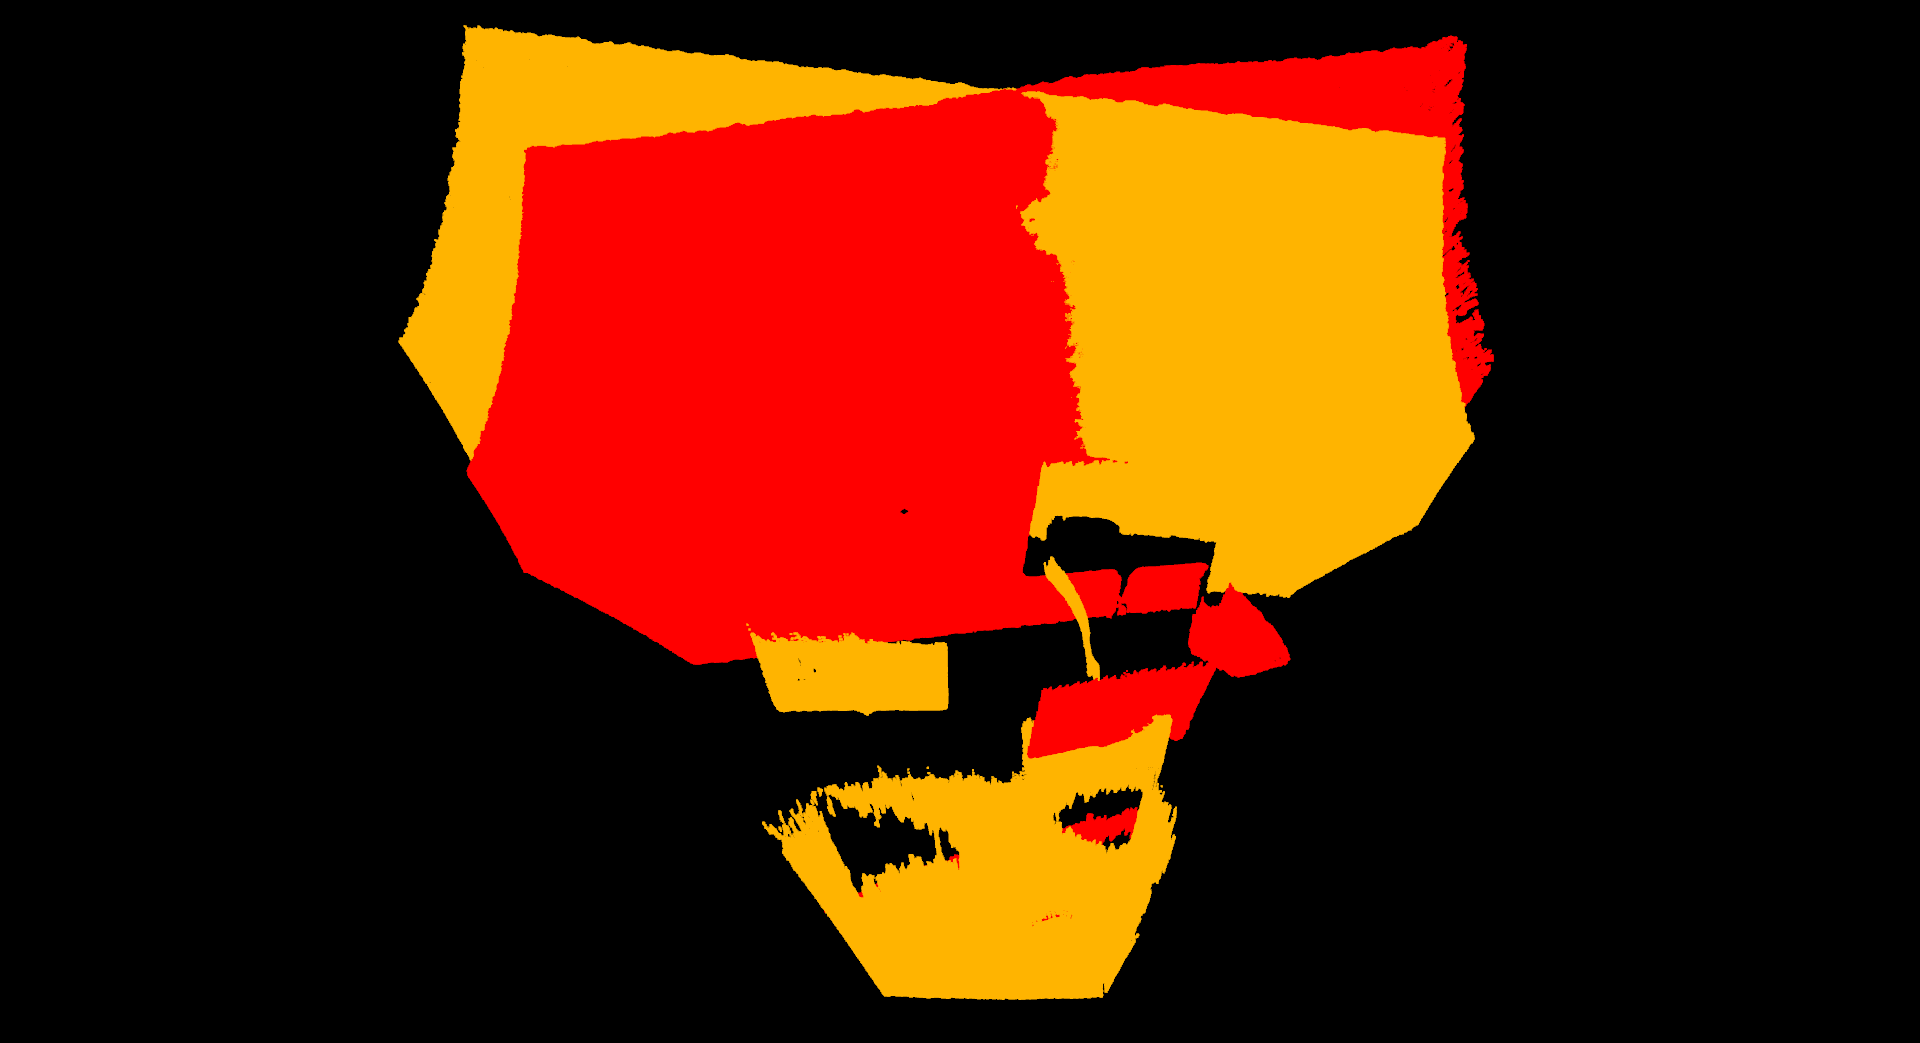
\includegraphics[width=\textwidth]{images/registration/pc_raw_static_merged_color.png}
    \caption{Red: point cloud 1. Yellow: point cloud 2.}
    \label{figure:pc_raw_static_merged_color}
  \end{subfigure}
  \caption{Merge of the two point clouds created from the two different views before applying any transformation. The point of view is virtual.}
  \label{figure:pc_raw_static_merged}
\end{figure}

Global registration procedure failed to find any transformation matrix to align the two point clouds of figure \ref{figure:pc_raw_static_merged}. One  reason could be the difficulty for FPFH to find relevant feature to process the alignment. As FPFH describes the local geometry property of a point, this property could be too much similar with point clouds having big planar surfaces.

\textbf{Experiment 2}

Applying the same procedure on the same scene but without the background (i.e. the wall) gives some results for the transformation matrix. The problem is that each time the global registration procedure is executed, the resulting output is extremely different and gives rarely a good result (about 1/20), see figure \ref{figure:ransac}. The reason is the RANSAC step where point are picked randomly and also because FPFH gives too similar local geometry properties.

\begin{figure}[H]
\centering
  \begin{subfigure}[b]{0.48 \textwidth}
    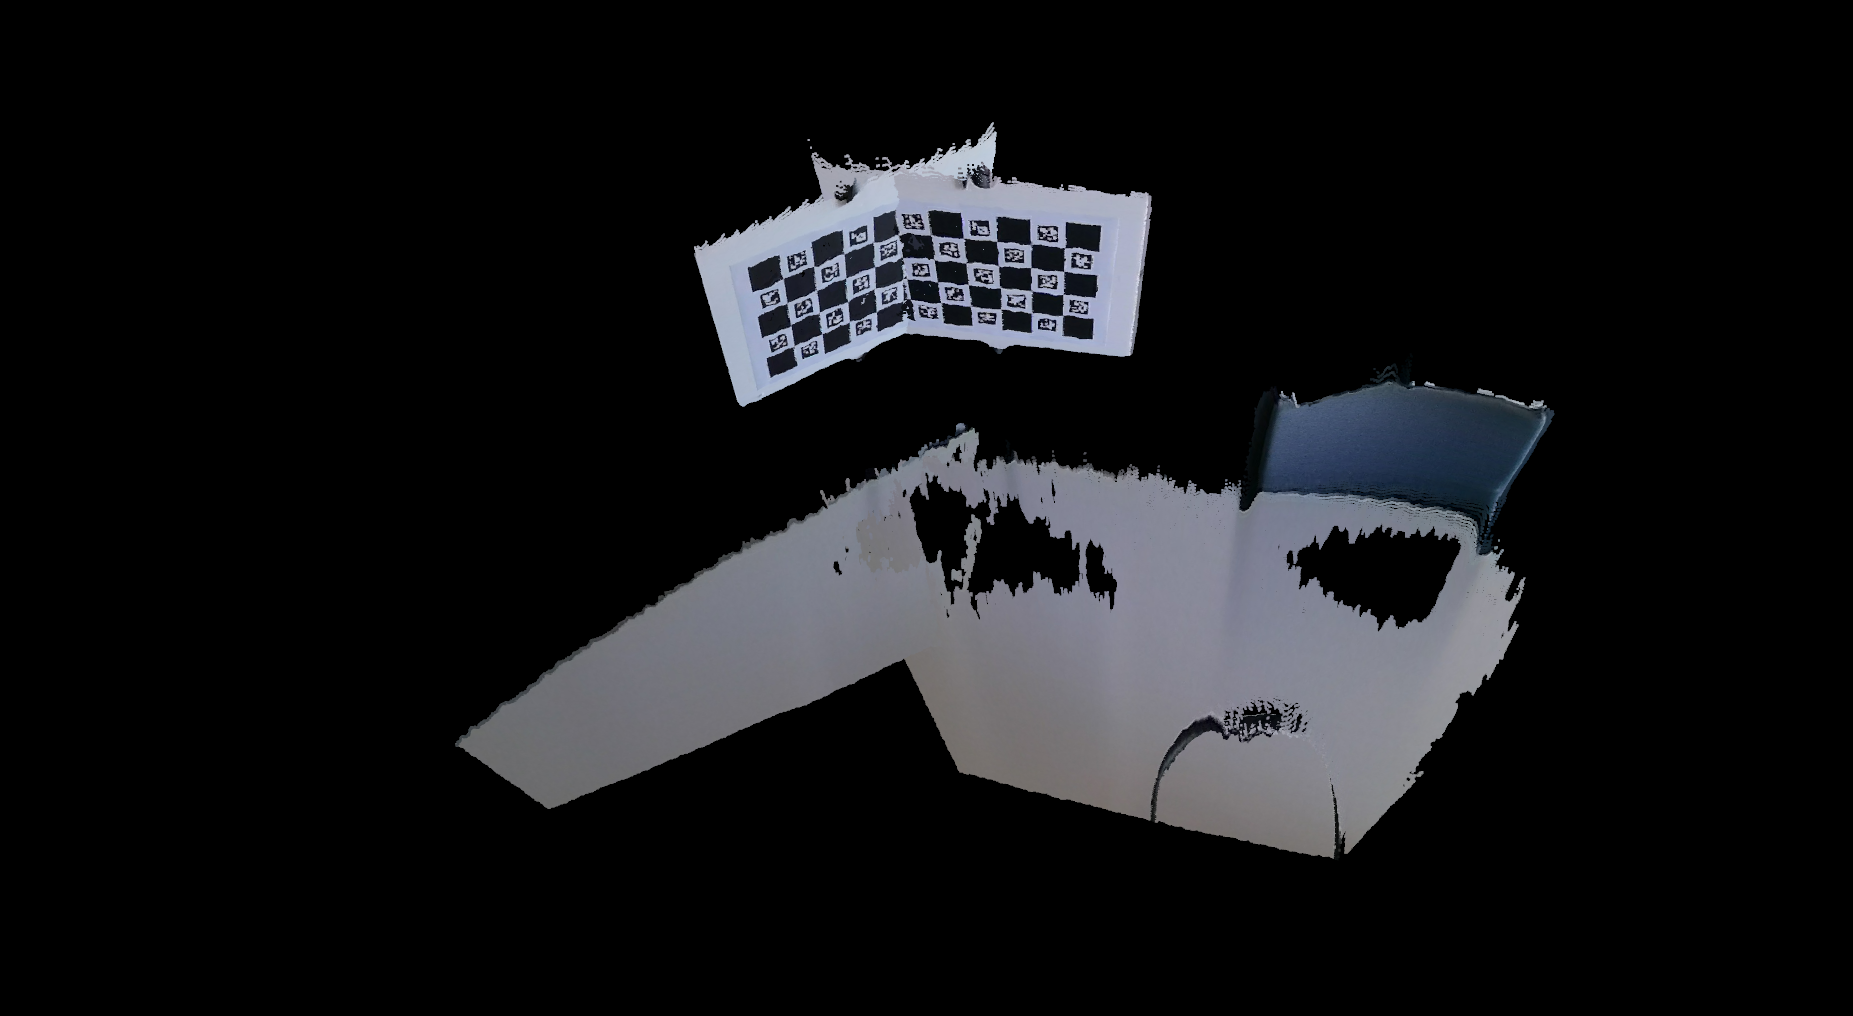
\includegraphics[width=\textwidth]{images/registration/ransac0.png}
    \caption{Example 1}
    \label{figure:ransac0}
  \end{subfigure}
  \hfill
  \begin{subfigure}[b]{0.48 \textwidth}
    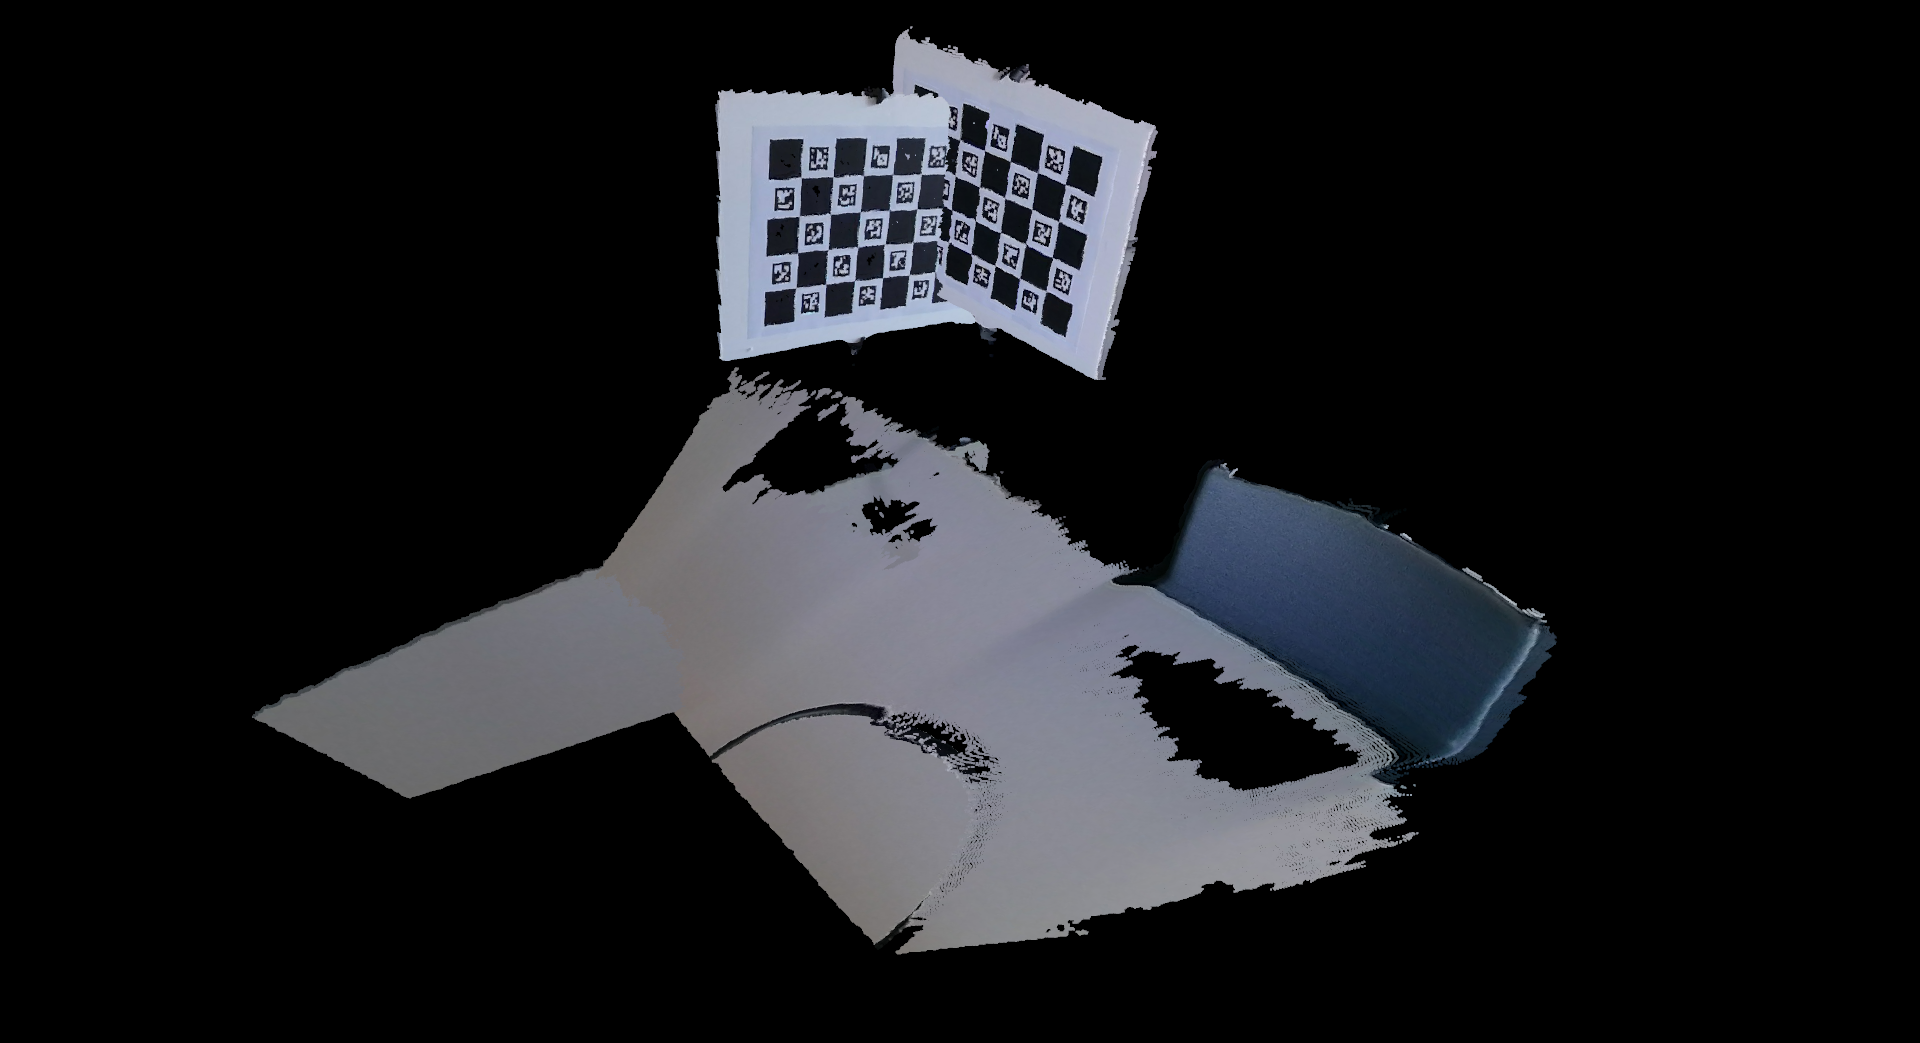
\includegraphics[width=\textwidth]{images/registration/ransac1.png}
    \caption{Example 2}
    \label{figure:ransac1}
  \end{subfigure}
  \caption{Sample of bad transformation matrix found by the global registration procedure}
  \label{figure:ransac}
\end{figure}

Figure \ref{figure:ransac_ok} shows an example where the global registration procedure succeeds to find an acceptable transformation matrix.

\begin{figure}[H]
\centering
  \begin{subfigure}[b]{0.48 \textwidth}
    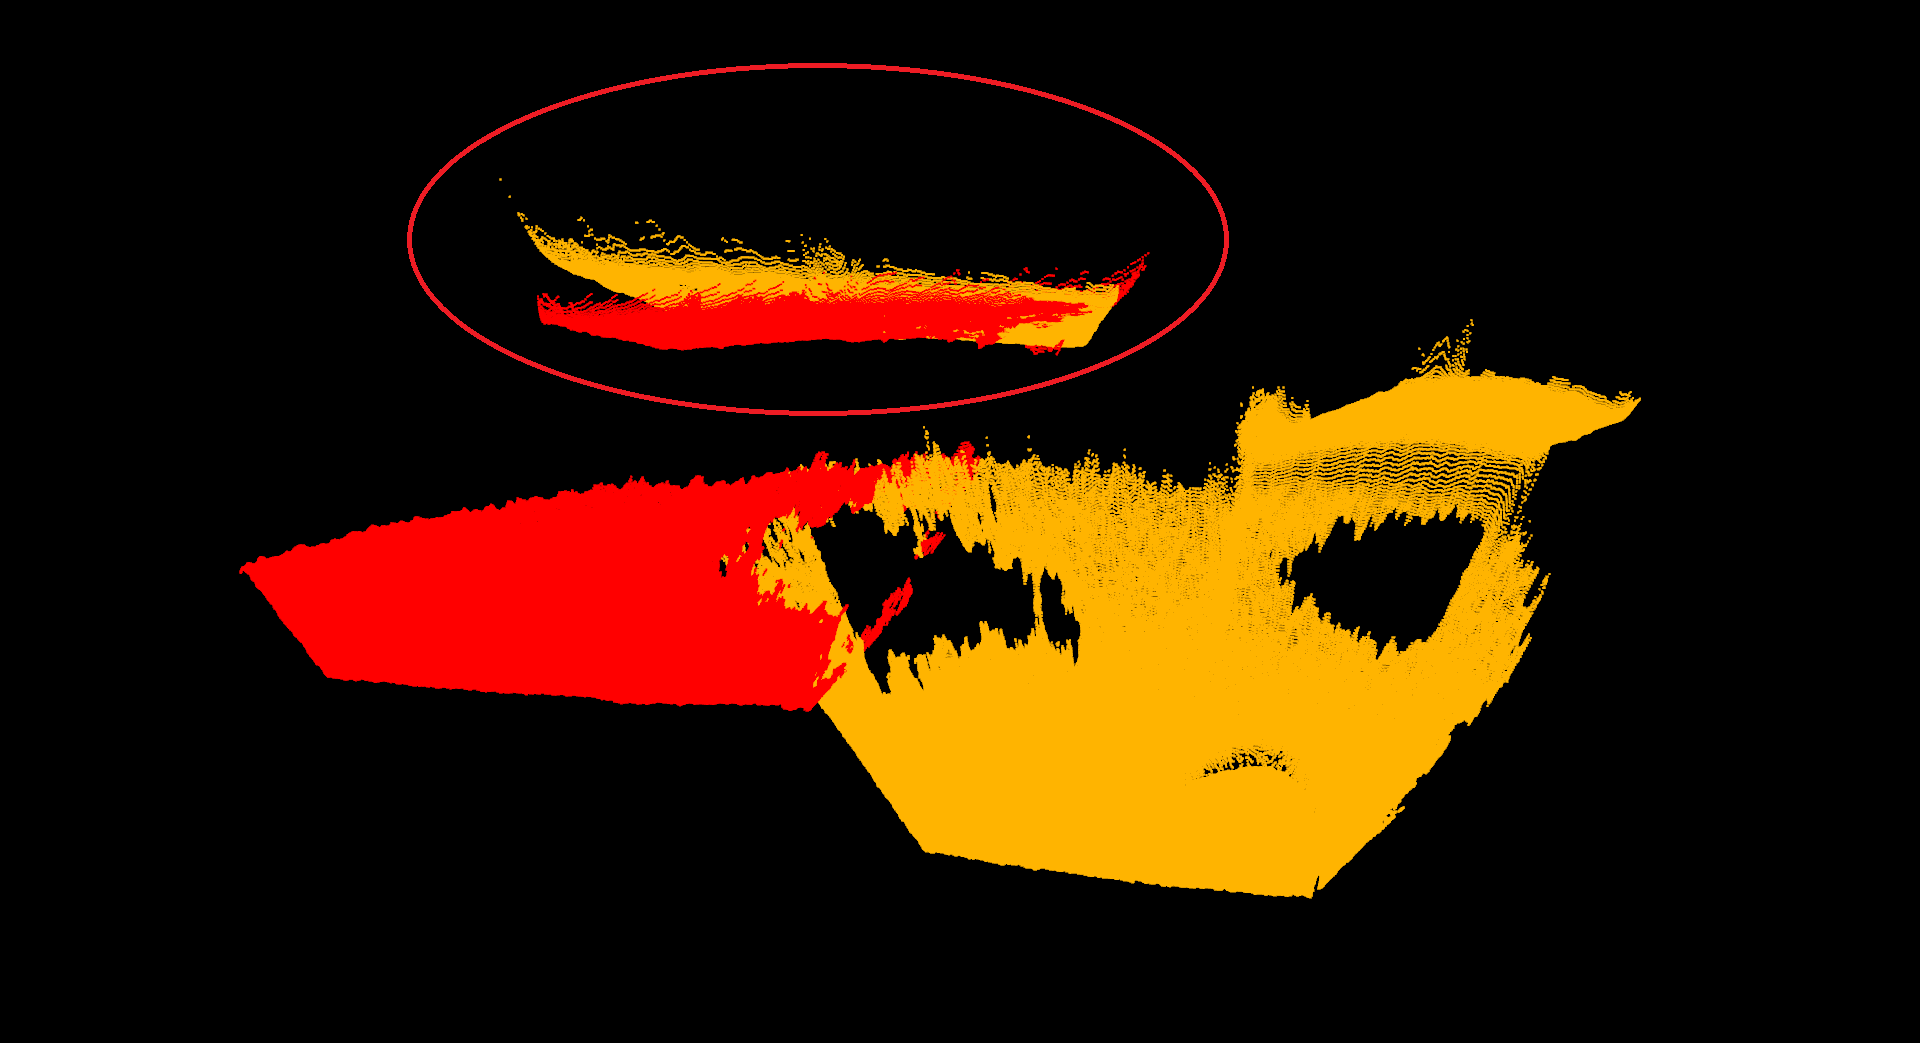
\includegraphics[width=\textwidth]{images/registration/ransac_ok_red.png}
    \caption{Result of the alignment after the RANSAC step}
    \label{figure:ransac_ok}
  \end{subfigure}
  \hfill
  \begin{subfigure}[b]{0.48 \textwidth}
    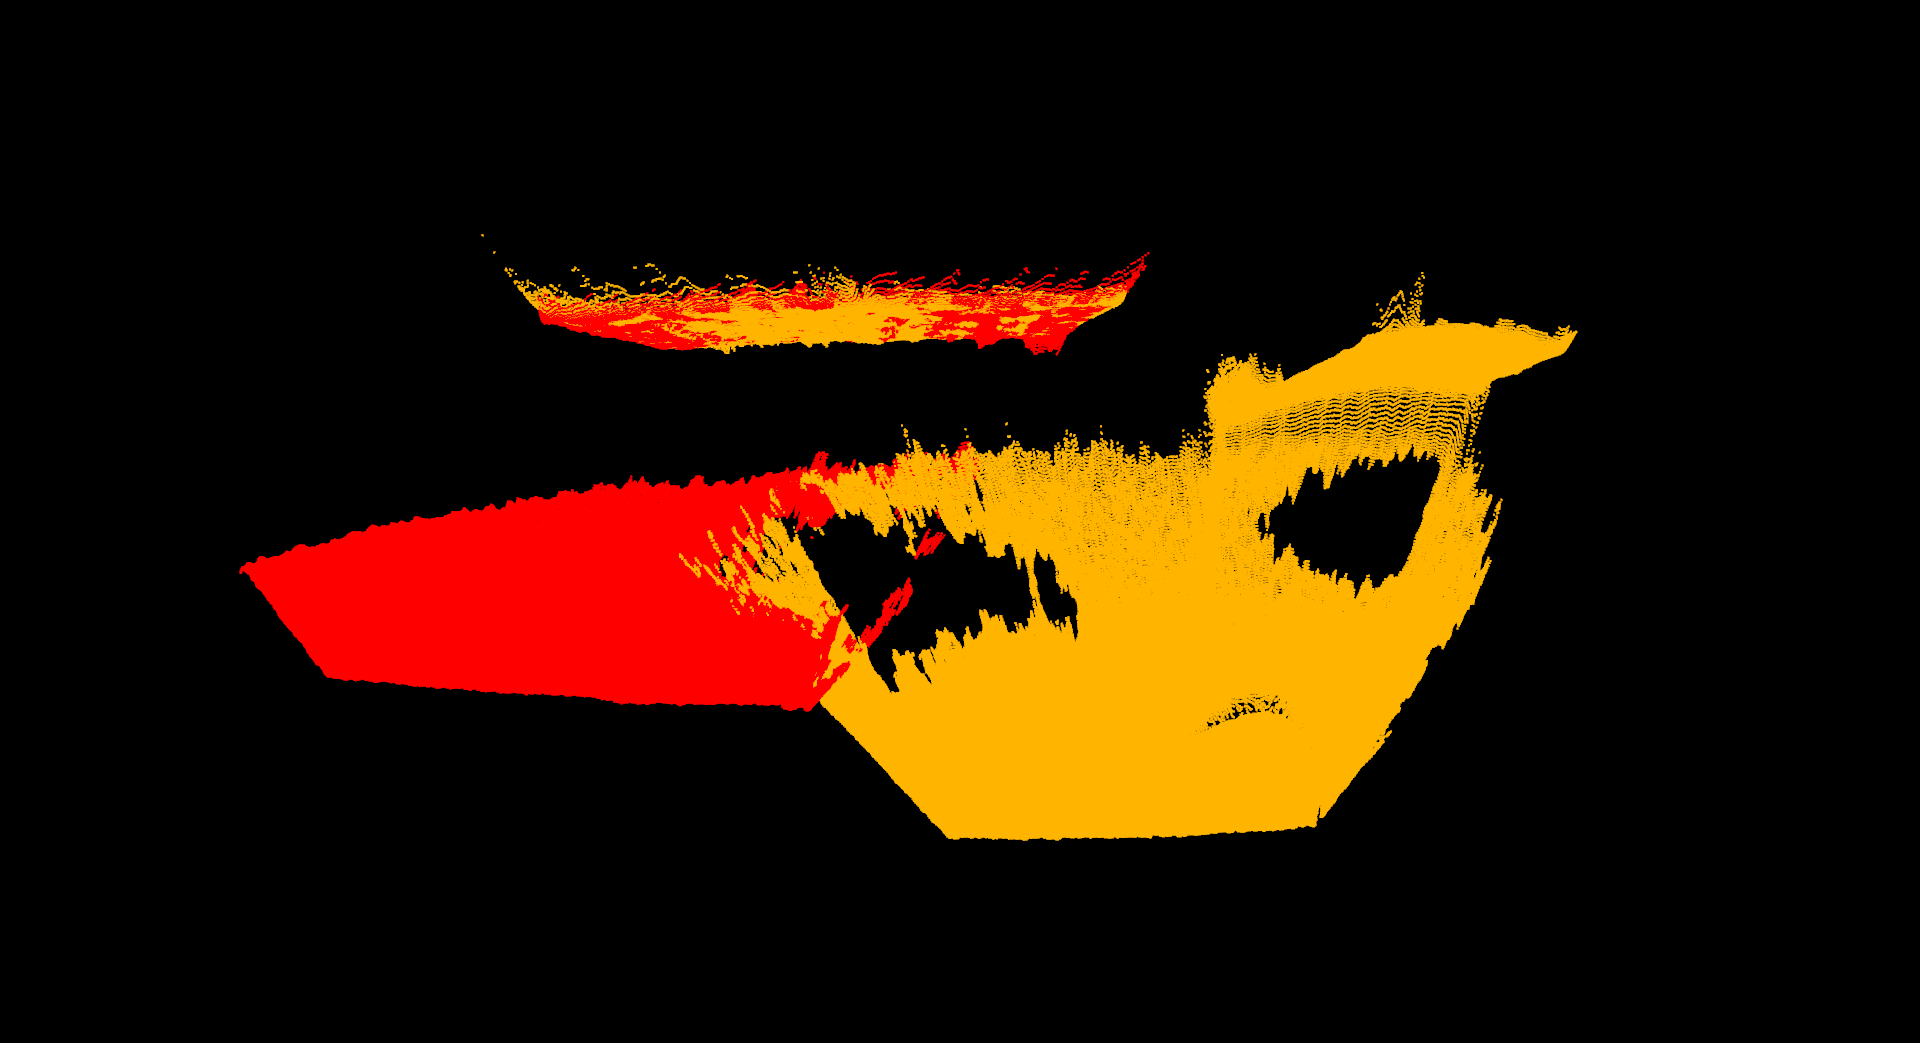
\includegraphics[width=\textwidth]{images/registration/ransac_icp_ok.png}
    \caption{Result of the alignment after the local refinement}
    \label{figure:ransac_icp_ok}
  \end{subfigure}
  \caption{Result of the global procedure on a sample without a wall as background. This is a virtual top view of the scene. Red: point cloud 1. Yellow: point cloud 2.}
  \label{figure:ransac_ok}
\end{figure}

Table \ref{tab:mae_global_registration_exp1} presents the result of applying the found transformation matrices on the  ChArUco board corners point clouds. It shows a non negligible improvement after the local refinement step.

\begin{table}[H]
\centering
\begin{tabular}{c|c|c|c}
 & \textbf{X - coordinate} & \textbf{Y - coordinate} & \textbf{Z - coordinate} \\ \hline
\textbf{\begin{tabular}[c]{@{}c@{}}Mean Absolute Error after\\ the RANSAC step {[}mm{]}\end{tabular}} & 6.05 & 13.14 & 20.11 \\ \hline
\textbf{\begin{tabular}[c]{@{}c@{}}Mean Absolute Error after\\ the refinement step {[}mm{]}\end{tabular}} & 3.04 & 0.57 & 2.40
\end{tabular}
\caption{Mean absolute error for the global registration experiment}
\label{tab:mae_global_registration_exp1}
\end{table}

\textbf{Experiment 3}

For this experiment, a scene with less planar surfaces is used. A static subject is put in the middle of the scene. Figure \ref{figure:raw_myself} shows the initial situation. The wall in the background is removed.

\begin{figure}[H]
\centering
  \begin{subfigure}[b]{0.48 \textwidth}
    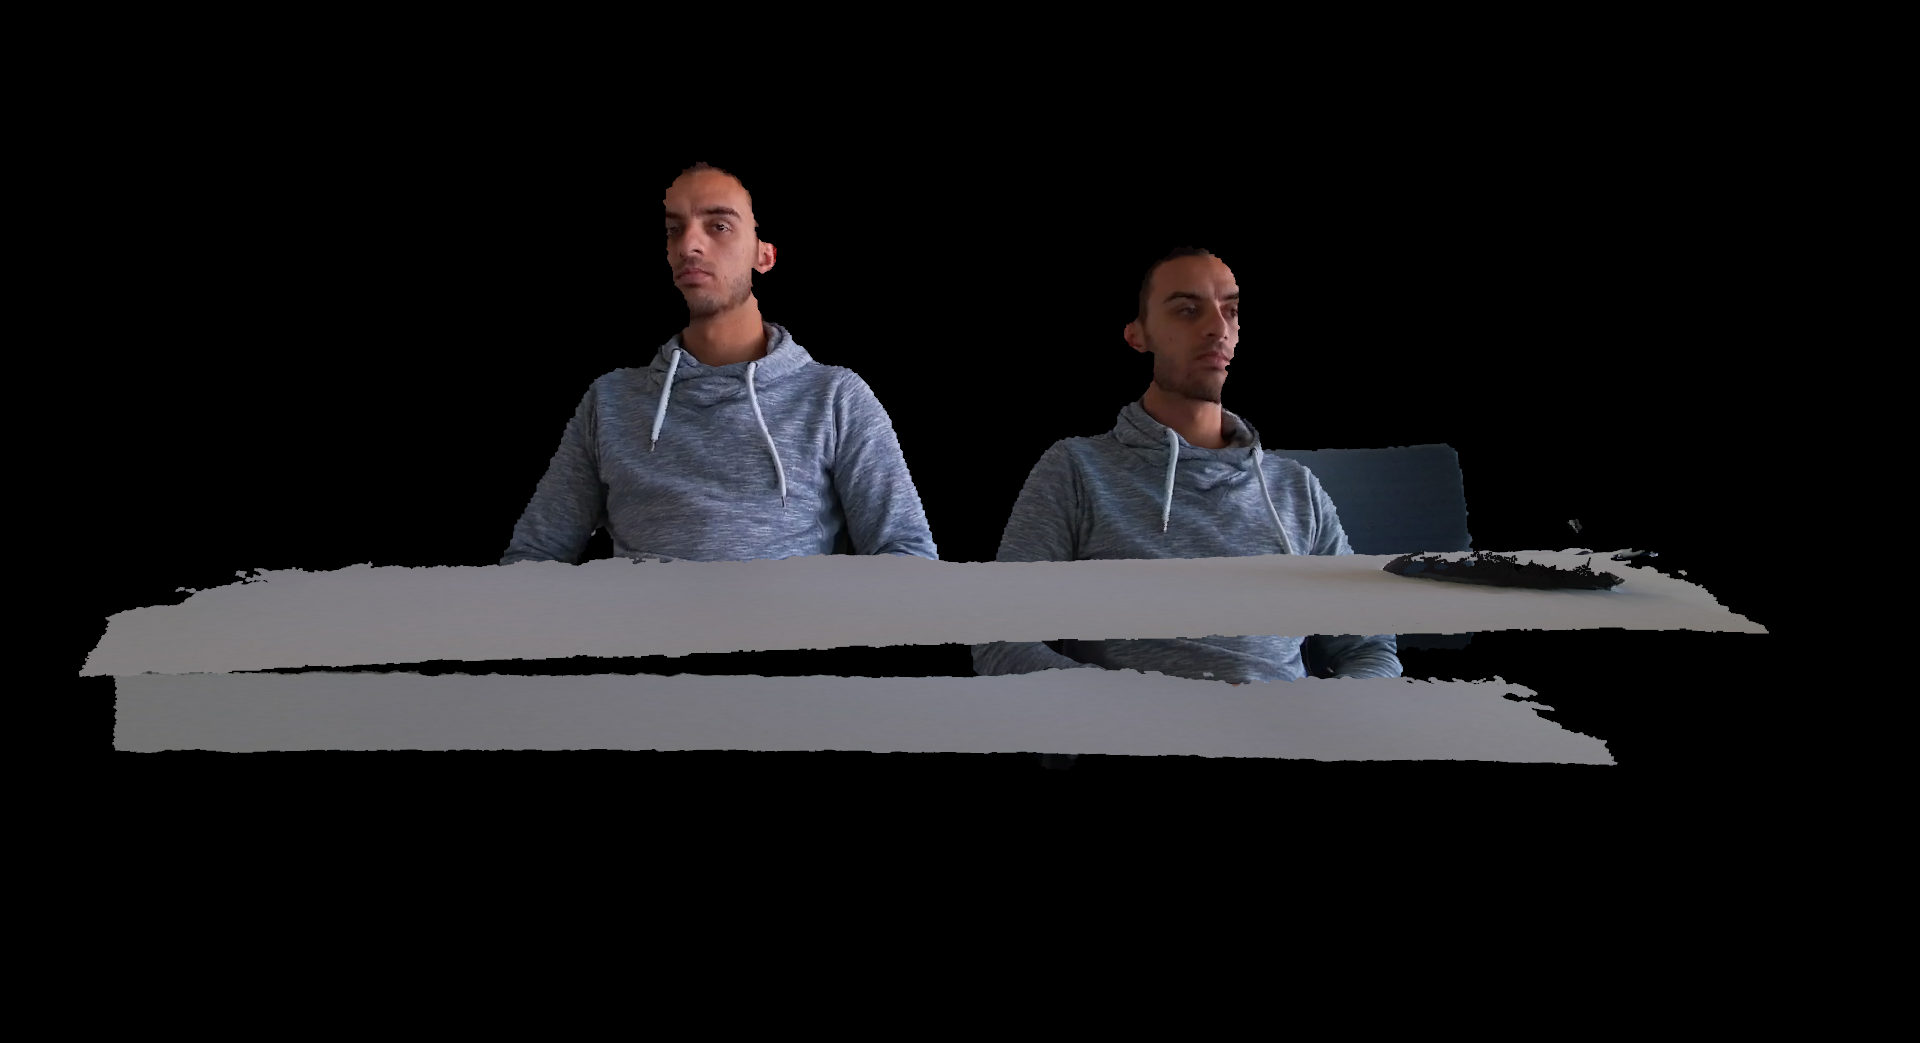
\includegraphics[width=\textwidth]{images/registration/raw_myself_RGB.png}
    \caption{RGB merged point clouds}
    \label{figure:raw_myself_RGB}
  \end{subfigure}
  \hfill
  \begin{subfigure}[b]{0.48 \textwidth}
    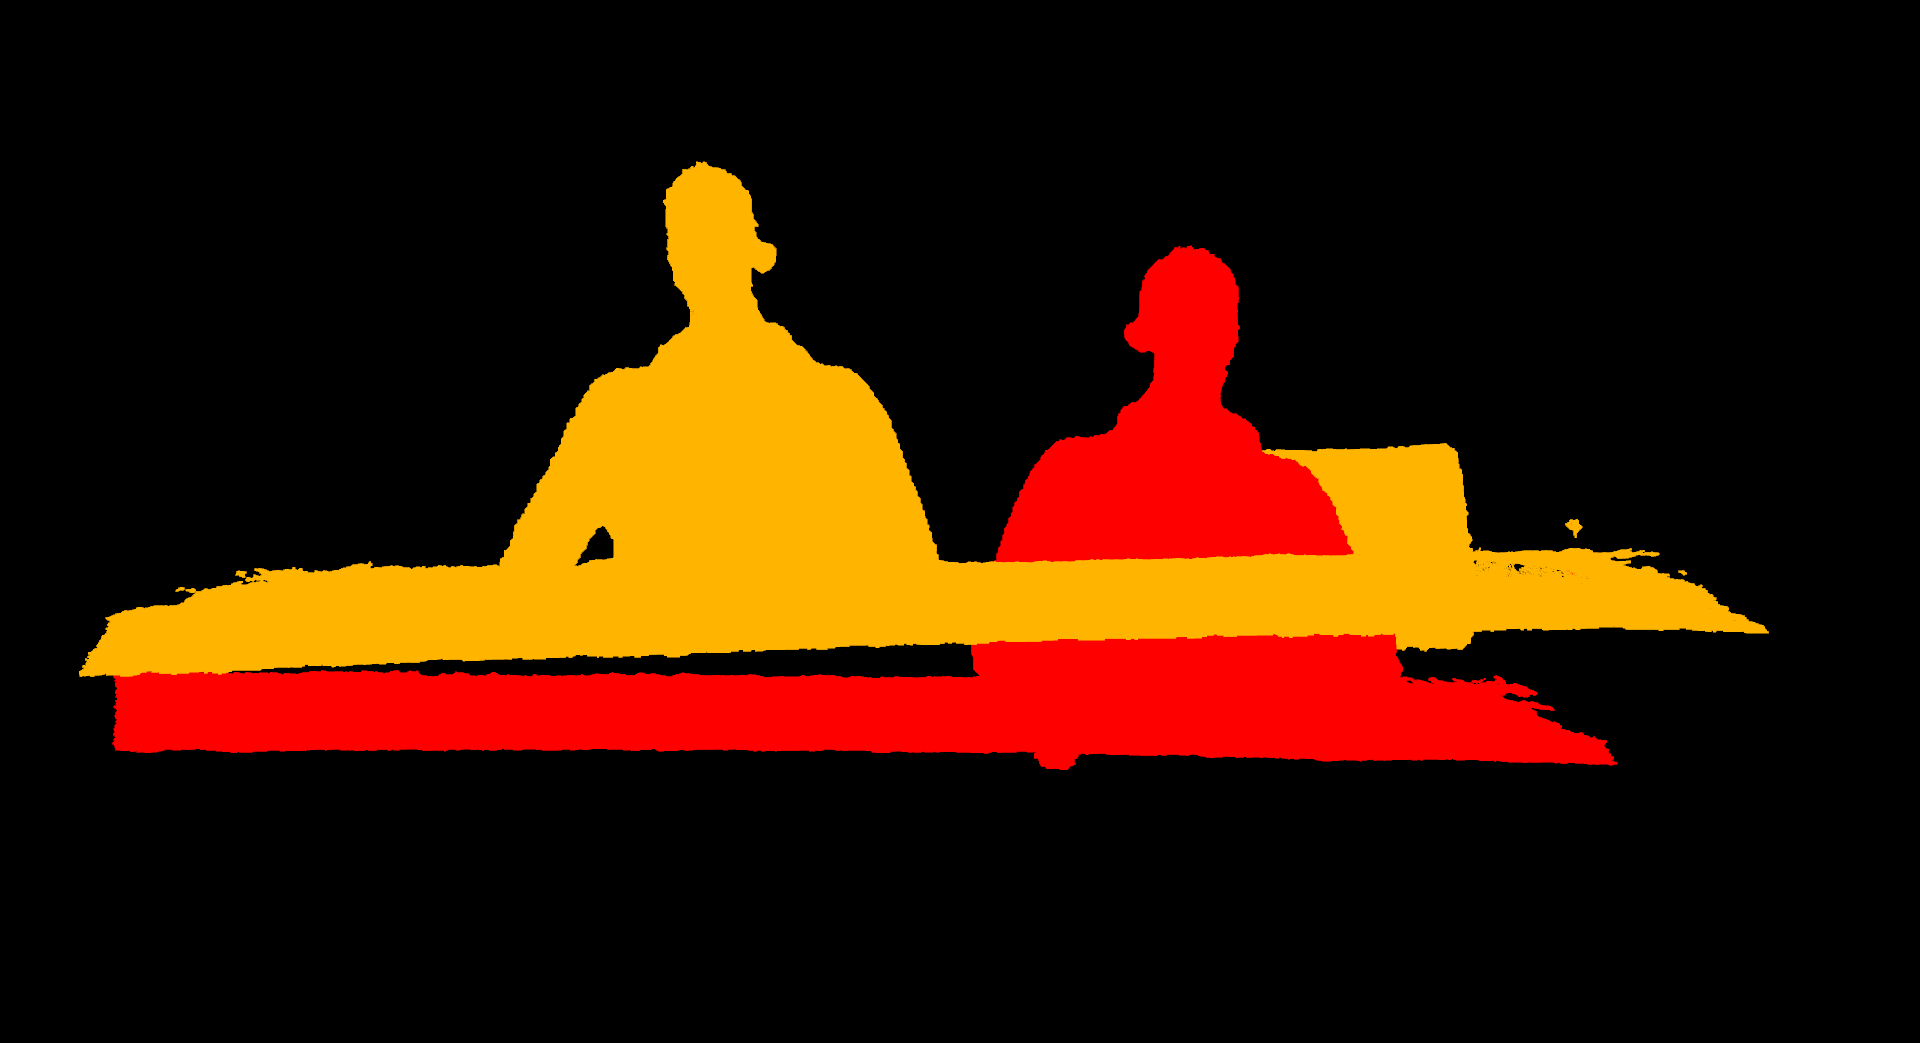
\includegraphics[width=\textwidth]{images/registration/raw_myself_colored.png}
    \caption{Red: point cloud 1. Yellow: point cloud 2.}
    \label{figure:raw_myself_colored}
  \end{subfigure}
  \caption{Merge of the two point clouds created from the two different views before applying any transformation. The point of view is virtual.}
  \label{figure:raw_myself}
\end{figure}

The global registration algorithm finds an acceptable transformation matrix each time. However, because of the randomness of the RANSAC step, the found transformation matrix is slightly different each time the procedure is launched. Figure \ref{figure:ransac_refine_myself_RGB} shows the alignment after the RANSAC step and the refinement step, respectively figure \ref{figure:ransac_myself_RGB} and \ref{figure:refine_myself_RGB}.

\begin{figure}[H]
\centering
  \begin{subfigure}[b]{0.48 \textwidth}
    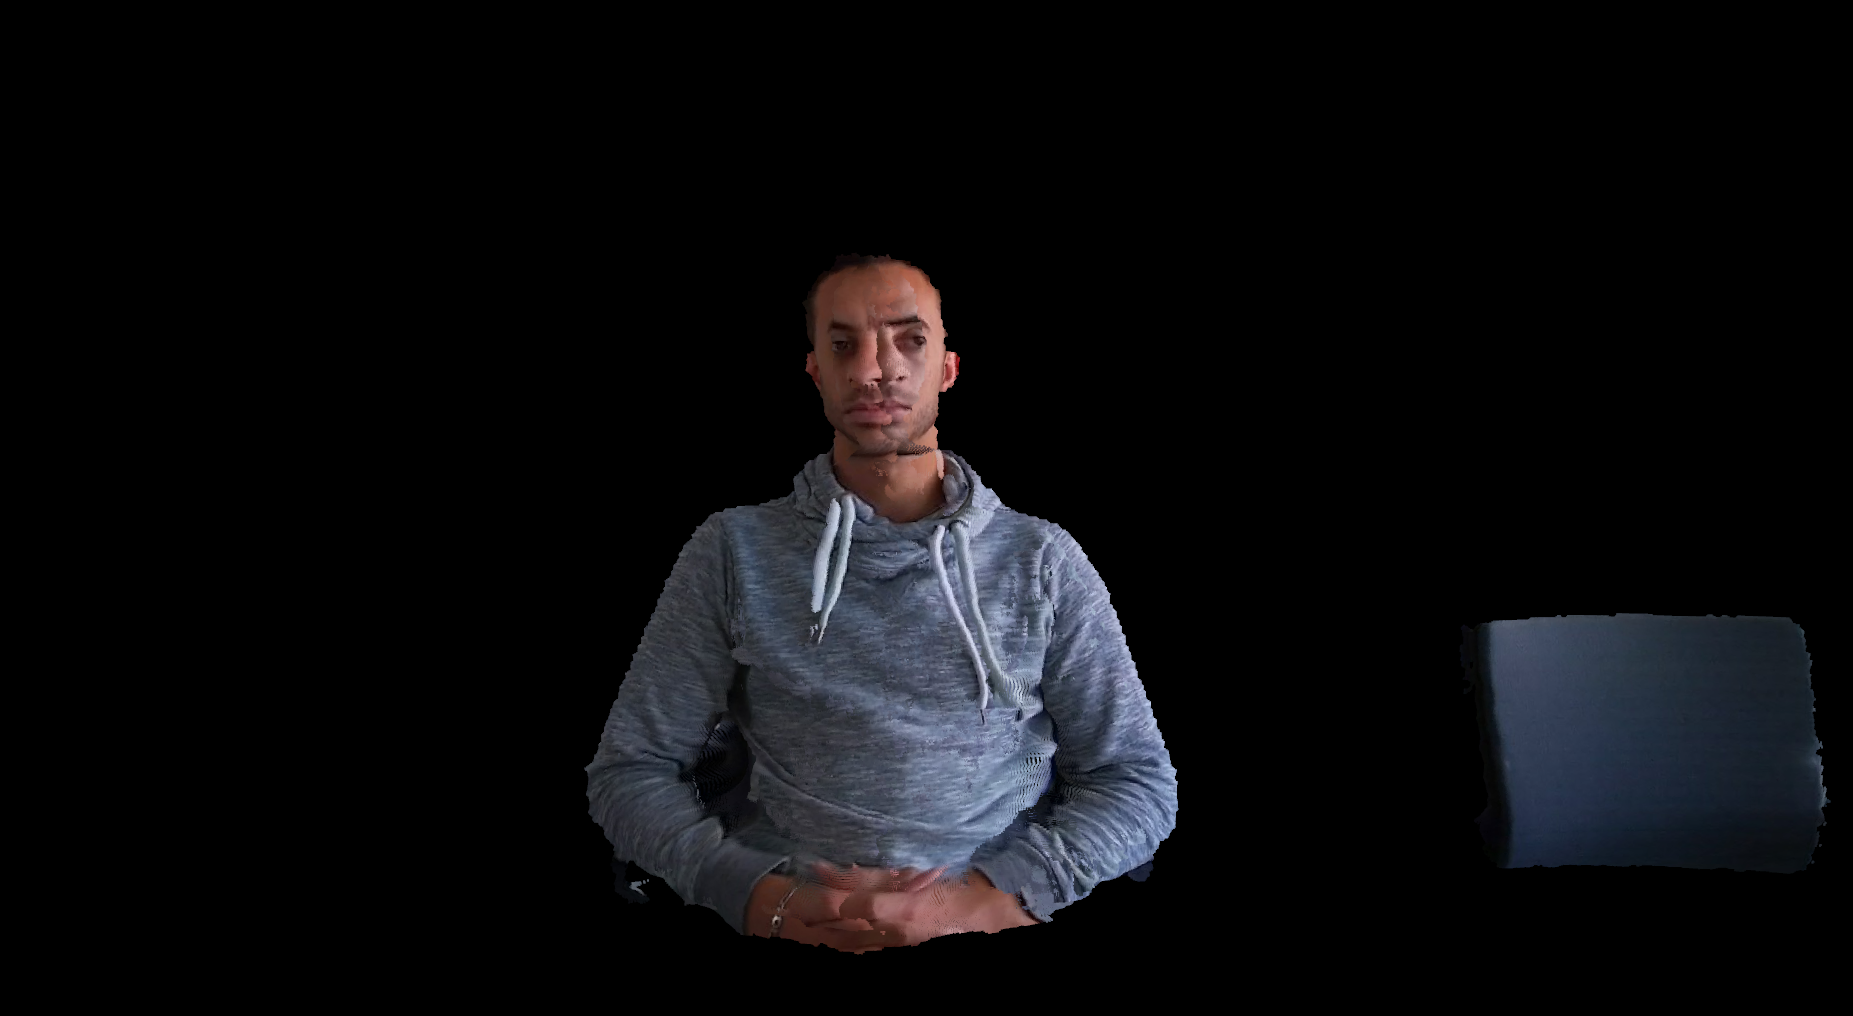
\includegraphics[width=\textwidth]{images/registration/ransac_myself_RGB.png}
    \caption{Alignment after the RANSAC step}
    \label{figure:ransac_myself_RGB}
  \end{subfigure}
  \hfill
  \begin{subfigure}[b]{0.48 \textwidth}
    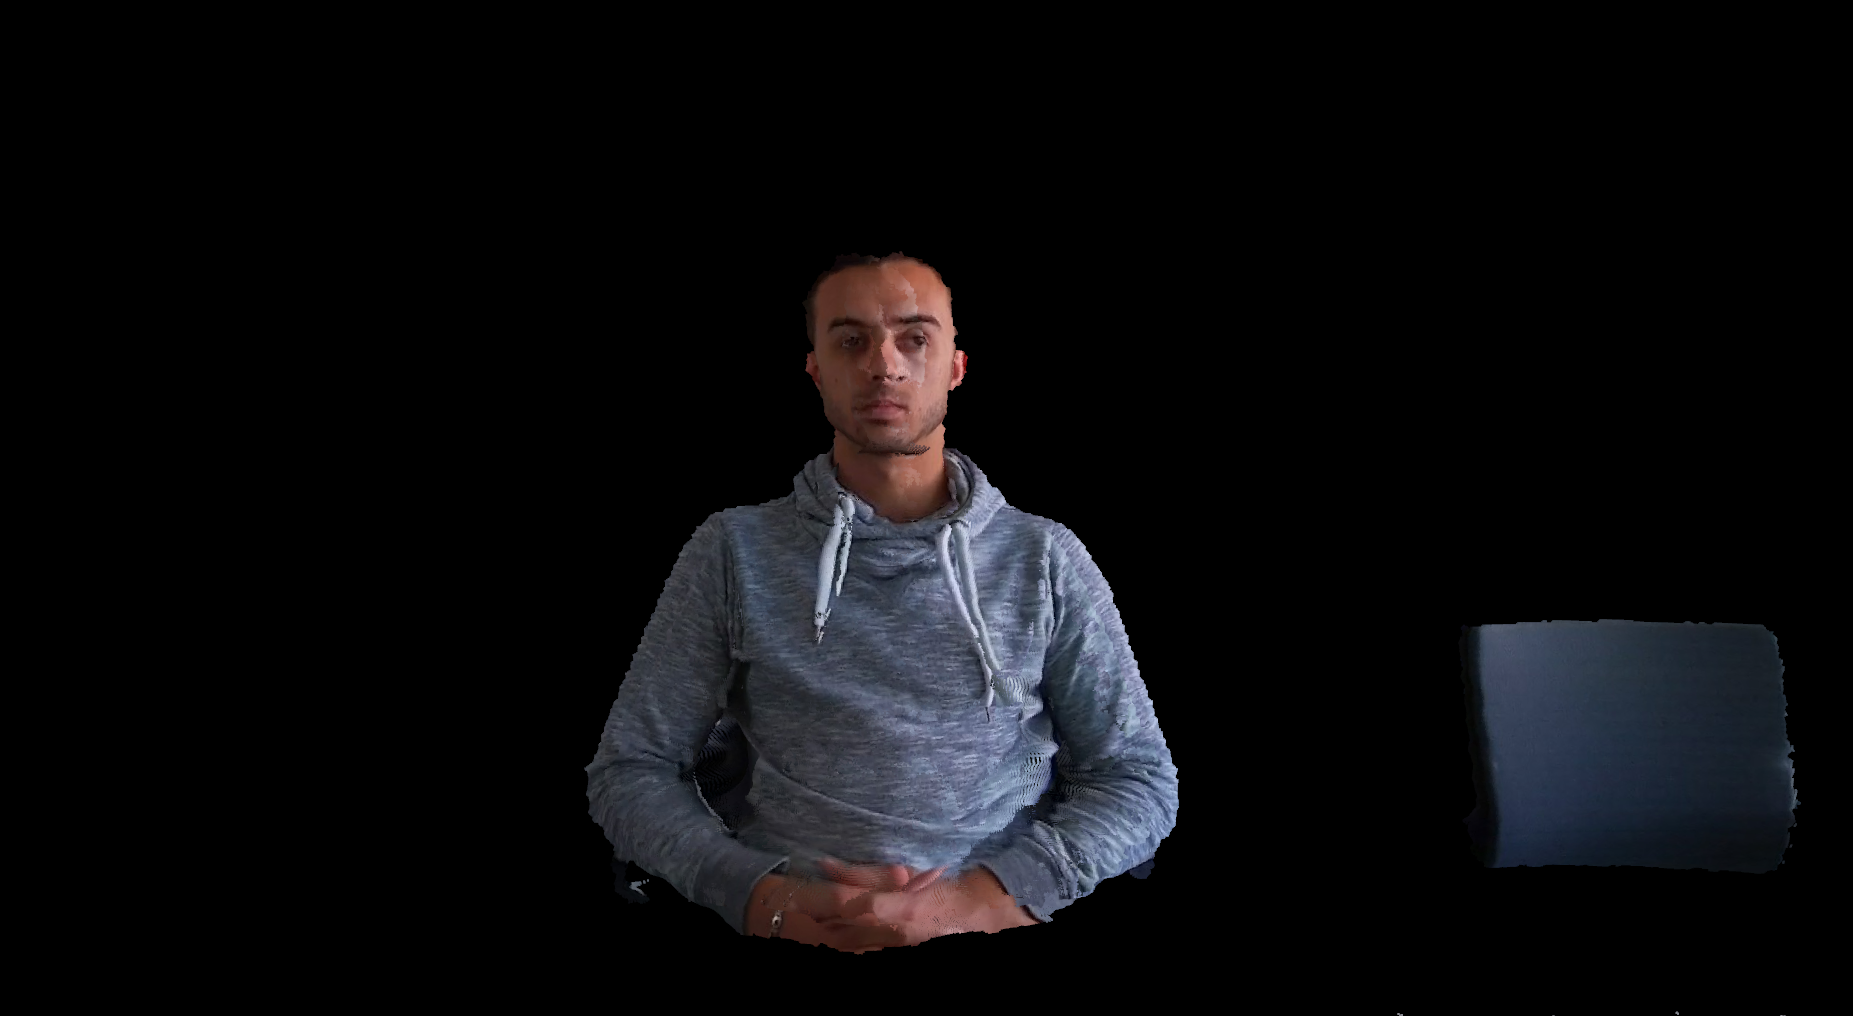
\includegraphics[width=\textwidth]{images/registration/refine_myself_RGB.png}
    \caption{Alignment after the refine step}
    \label{figure:refine_myself_RGB}
  \end{subfigure}
  \caption{Alignment of the two point clouds created from the two different views. The point of view is virtual.}
  \label{figure:ransac_refine_myself_RGB}
\end{figure}

Table \ref{tab:mae_global_registration_exp3} presents the results the three different matrices, found in the three previous experiments, applied on one of the ChArUco board point clouds of figure \ref{figure:pc_arucoboard}. One can notice that the result of the RANSAC step is not good enough to find an accurate transformation. The refinement step brings improvement. However, in this experiment, the MAE in \textit{X} is still high and noticeable in a live video demonstration. 


% Please add the following required packages to your document preamble:
% \usepackage{multirow}
\begin{table}[H]
\centering
\begin{tabular}{c|c|c|c|c}
 & \textbf{Run} & \textbf{X - coordinate} & \textbf{Y - coordinate} & \textbf{Z - coordinate} \\ \hline
\multirow{3}{*}{\textbf{\begin{tabular}[c]{@{}c@{}}Mean Absolute Error\\ after the RANSAC\\ step {[}mm{]}\end{tabular}}} & 1 & 30.67 & 4.07 & 3.66 \\
 & 2 & 19.93 & 0.87 & 2.62 \\
 & 3 & 29.51 & 0.62 & 5.42 \\ \hline
\multirow{3}{*}{\textbf{\begin{tabular}[c]{@{}c@{}}Mean Absolute Error\\ after the refinement\\  step {[}mm{]}\end{tabular}}} & 1 & 13.82 & 1.29 & 1.27 \\
 & 2 & 13.81 & 1.29 & 1.27 \\
 & 3 & 13.81 & 1.29 & 1.44
\end{tabular}
\caption{Mean absolute error for the global registration experiment}
\label{tab:mae_global_registration_exp3}
\end{table}


\subsubsection{Iterative closest point registration}

For all the ICP algorithms presented in section \ref{section:Iterative closest point registration}, the critical point is the guessed initialisation matrix. As is it difficult to estimate it, the transformation found after the RANSAC step of the experiment 2 of the section \ref{section:Global registration result} is used for the initialisation step.

\textbf{Experiment 1}

Figure \ref{figure:init_ransac} shows the scene after applying the RANSAC transformation found. All ICP algorithms are applied to this initial transformed scene.

\begin{figure}[H]
\centering
  \begin{subfigure}[b]{0.48 \textwidth}
    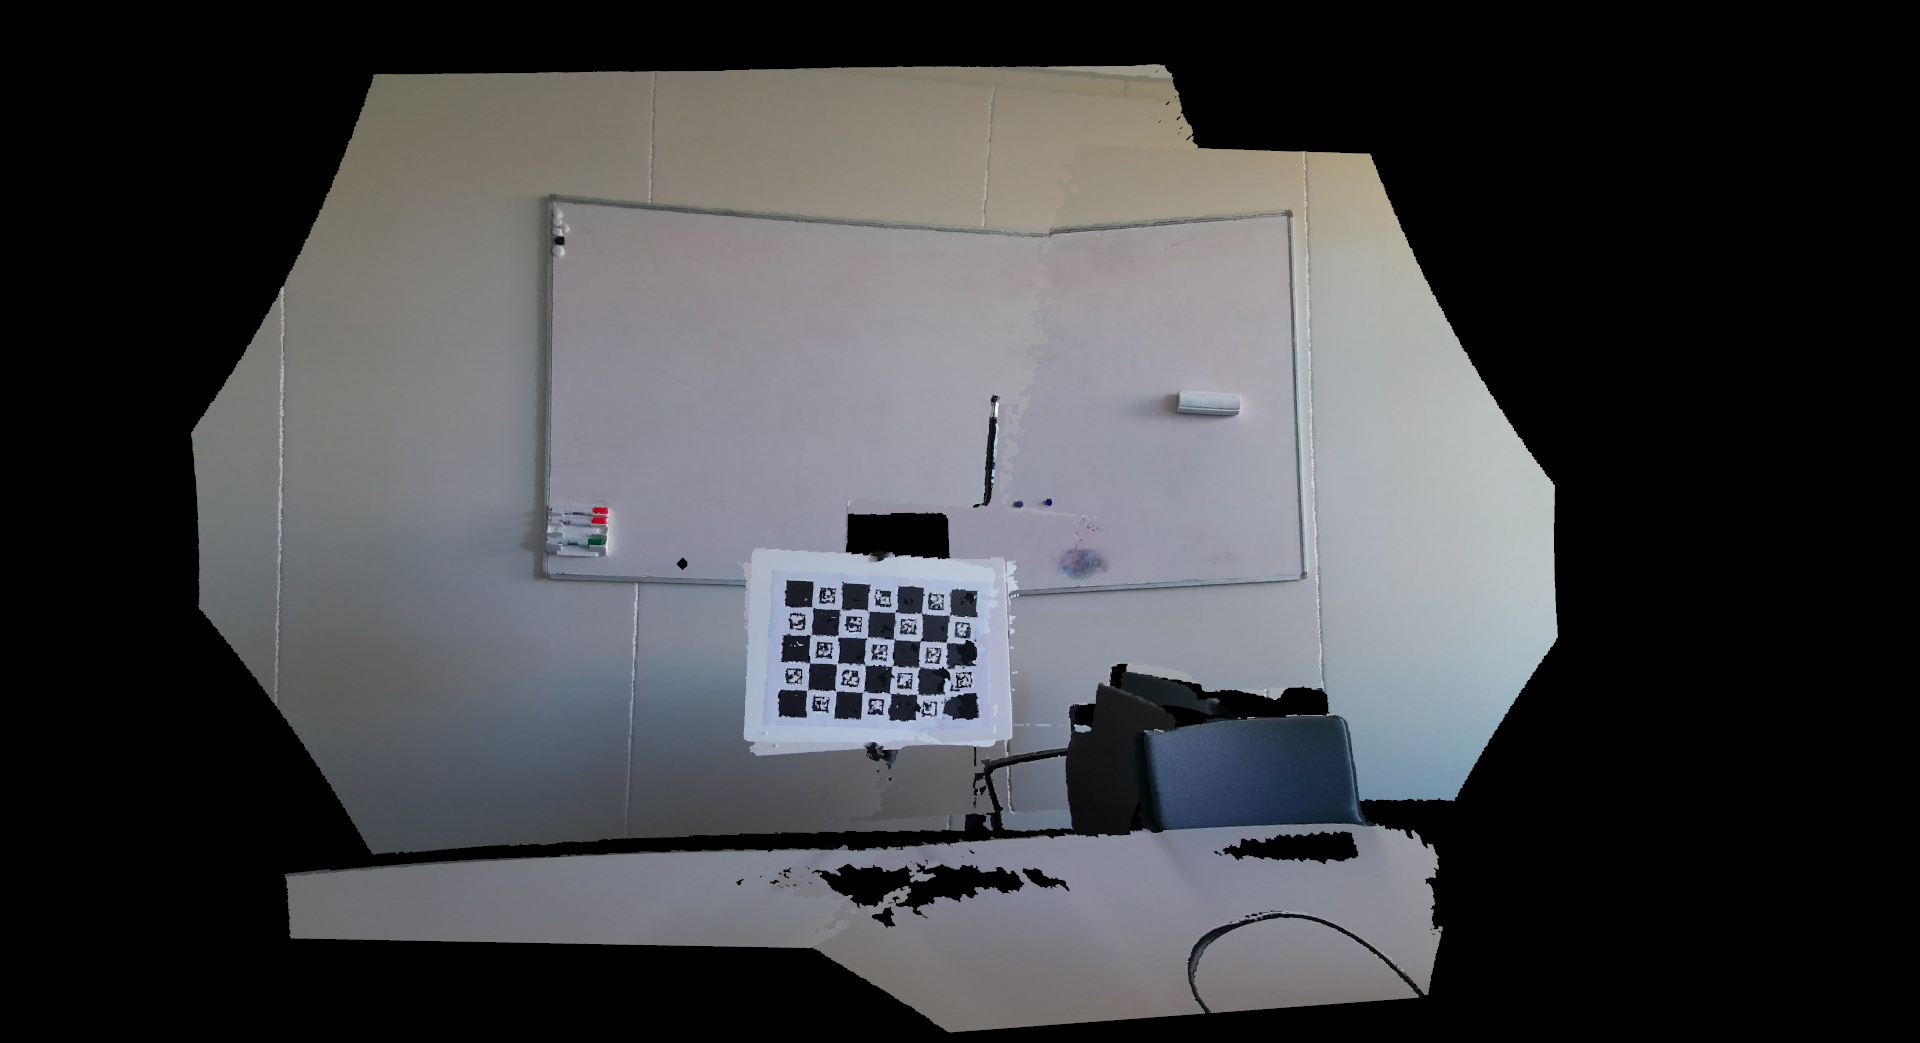
\includegraphics[width=\textwidth]{images/registration/init_ransac_RGB.png}
    \caption{Alignment after the RANSAC step}
    \label{figure:init_ransac_RGB}
  \end{subfigure}
  \hfill
  \begin{subfigure}[b]{0.48 \textwidth}
    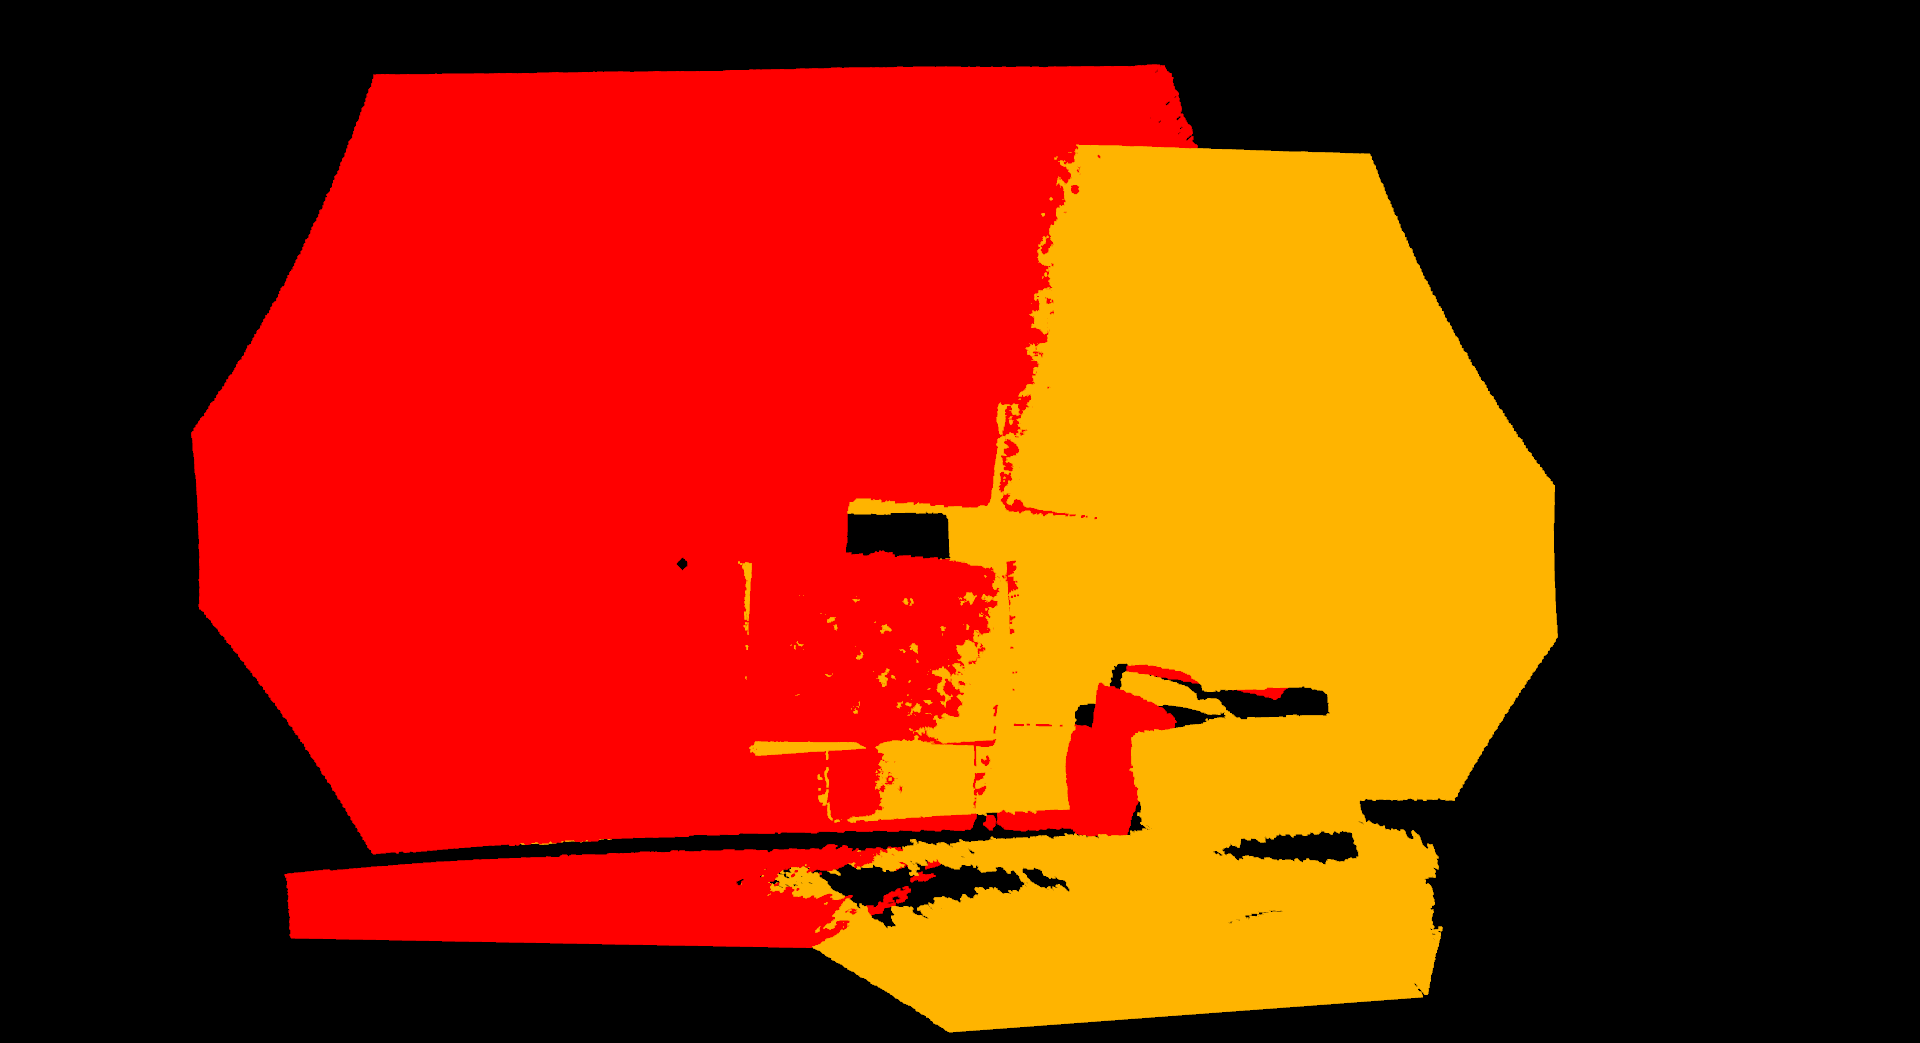
\includegraphics[width=\textwidth]{images/registration/init_ransac_colour.png}
    \caption{Alignment after the refine step}
    \label{figure:init_ransac_colour}
  \end{subfigure}
  \caption{Alignment of the two point clouds created from the two different views after the initialisation. The initialisation is made with a transformation matrix found by a RANSAC step. The point of view is virtual}
  \label{figure:init_ransac}
\end{figure}

Table \ref{tab:icp_1} shows the result of the different ICP methods. The colour registration method gives the best result. Taking into account the colour to find the transformation matrix helps the ICP algorithm. In opposite, point-to-point ICP doesn't improve the result of the initial step.

\begin{table}[H]
\begin{tabular}{c|c|c|c}
 & \textbf{X - coordinate} & \textbf{Y - coordinate} & \textbf{Z - coordinate} \\ \hline
\textbf{\begin{tabular}[c]{@{}c@{}}Mean Absolute Error\\ intial {[}mm{]}\end{tabular}} & 6.05 & 13.14 & 20.11 \\ \hline
\textbf{\begin{tabular}[c]{@{}c@{}}Mean Absolute Error\\ point-to-plane ICP {[}mm{]}\end{tabular}} & 6.87 & 9.56 & 15.03 \\ \hline
\textbf{\begin{tabular}[c]{@{}c@{}}Mean Absolute Error\\ point-to-point ICP {[}mm{]}\end{tabular}} & 7.51 & 14.58 & 19.12 \\ \hline
\textbf{\begin{tabular}[c]{@{}c@{}}Mean Absolute Error\\ coloured ICP {[}mm{]}\end{tabular}} & 2.17 & 2.67 & 2.51
\end{tabular}
\caption{Mean absolute error for the different ICP methods}
\label{tab:icp_1}
\end{table}

\textbf{Experiment 2}

For this experiment, the wall in the background is removed. Figure \ref{figure:init_ransac_crop} shows the initial situation before  launching the different ICP methods.

\begin{figure}[H]
\centering
  \begin{subfigure}[b]{0.48 \textwidth}
    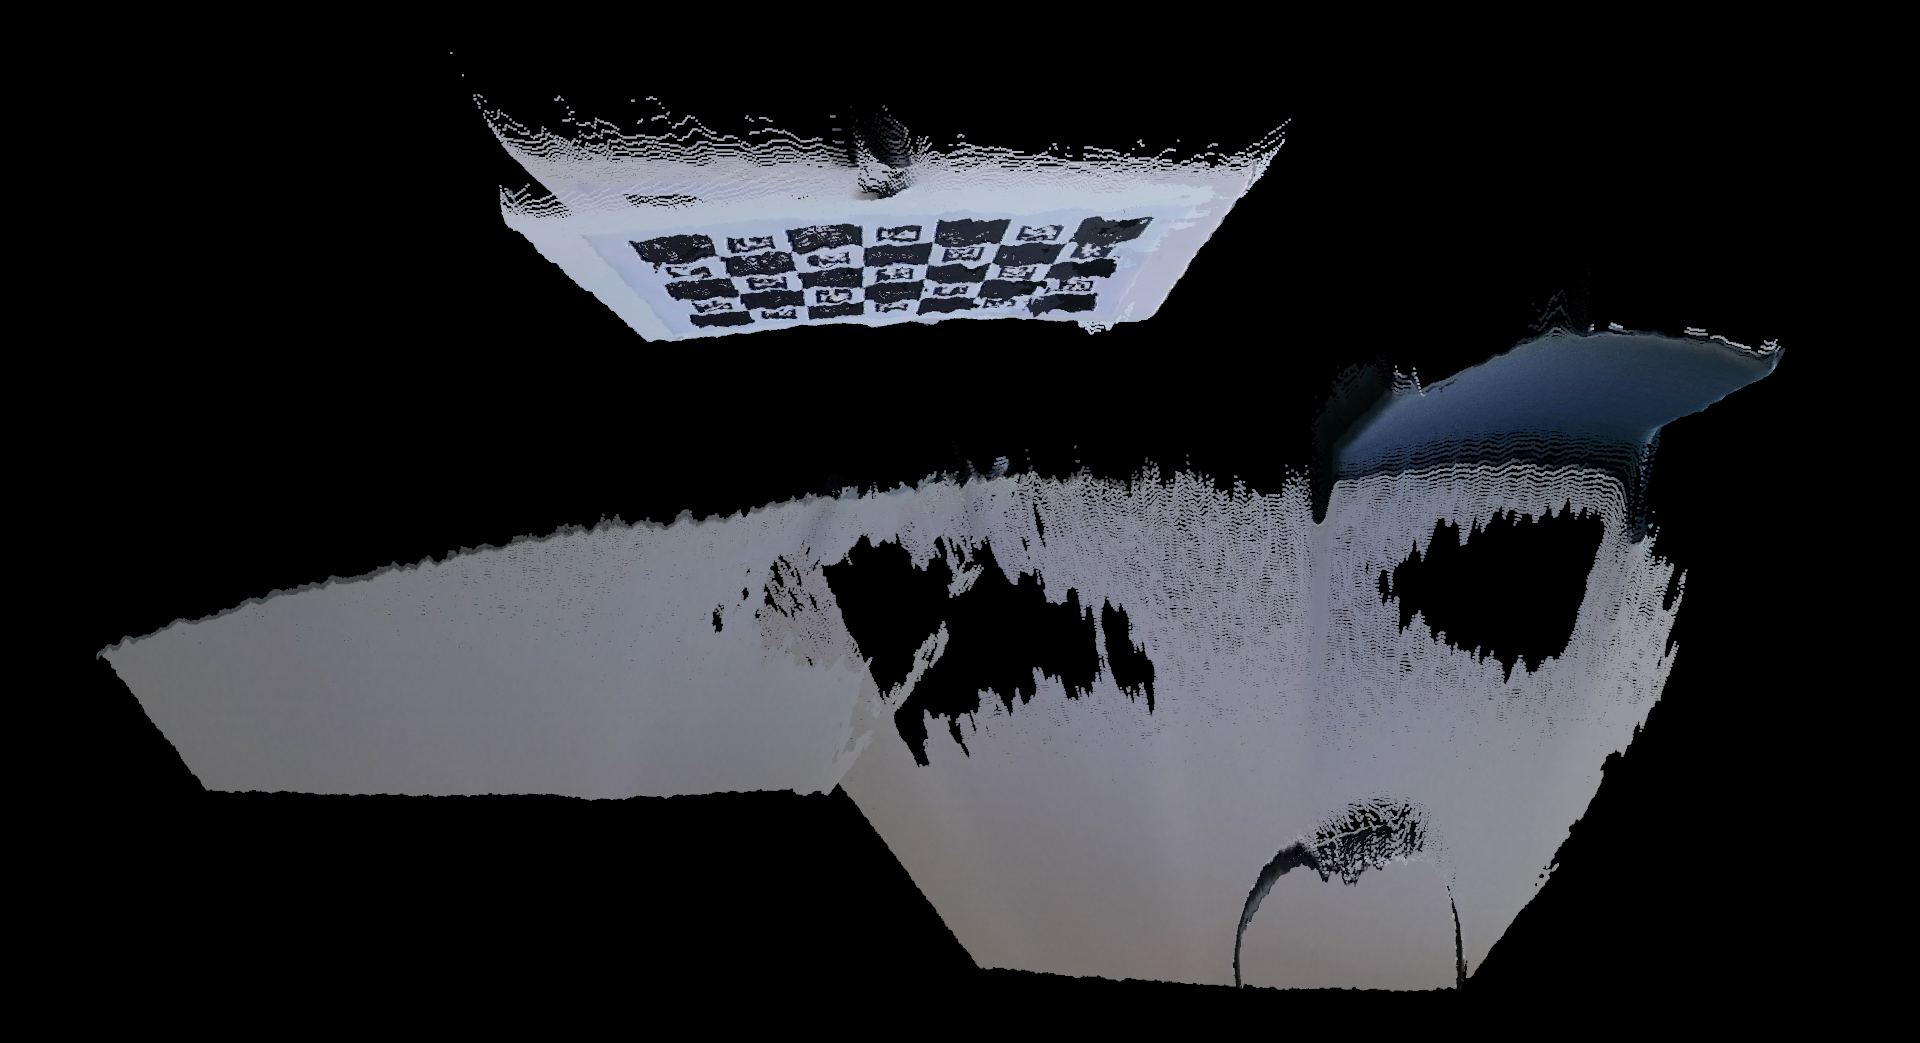
\includegraphics[width=\textwidth]{images/registration/init_ransac_crop_RGB.png}
    \caption{Alignment after the initialisationn}
    \label{figure:init_ransac_crop_RGB}
  \end{subfigure}
  \hfill
  \begin{subfigure}[b]{0.48 \textwidth}
    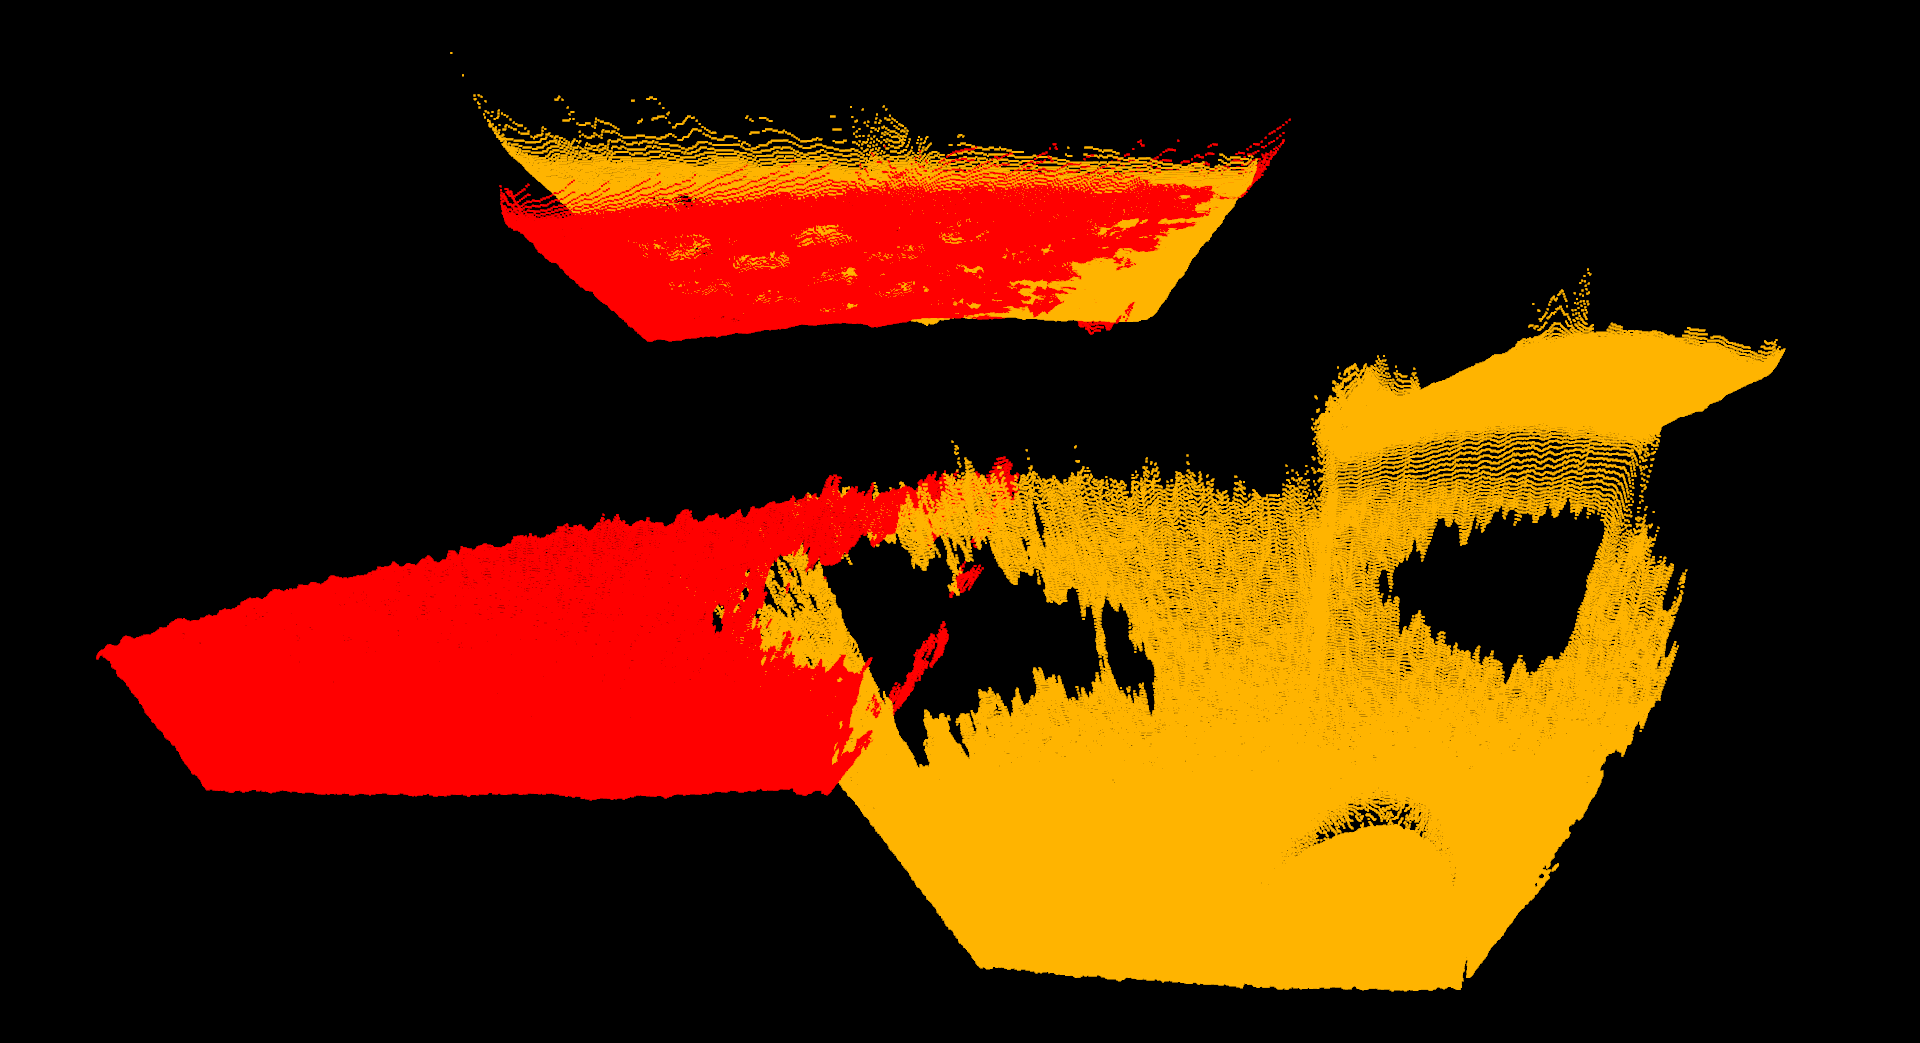
\includegraphics[width=\textwidth]{images/registration/init_ransac_crop_colour.png}
    \caption{Red: point cloud 1. Yellow: point cloud 2.}
    \label{figure:init_ransac_crop_colour}
  \end{subfigure}
  \caption{Alignment of the two point clouds created from the two different views after the initialisation. The initialisation is made with a transformation matrix found by a RANSAC step. The point of view is virtual.}
  \label{figure:init_ransac_crop}
\end{figure}

Table \ref{tab:icp_2} presents the result of the different ICP methods tried. The same observation as in experiment 1 can be made. Point-to-point ICP doesn't improve much the initial result. Coloured registration gives the best result. The colour information helps especially in the case of flat surfaces. 

\begin{table}[H]
\begin{tabular}{c|c|c|c}
 & \textbf{X - coordinate} & \textbf{Y - coordinate} & \textbf{Z - coordinate} \\ \hline
\textbf{\begin{tabular}[c]{@{}c@{}}Mean Absolute Error\\ intial {[}mm{]}\end{tabular}} & 6.05 & 13.14 & 20.11 \\ \hline
\textbf{\begin{tabular}[c]{@{}c@{}}Mean Absolute Error\\ point-to-plane ICP {[}mm{]}\end{tabular}} & 3.58 & 5.88 & 7.11 \\ \hline
\textbf{\begin{tabular}[c]{@{}c@{}}Mean Absolute Error\\ point-to-point ICP {[}mm{]}\end{tabular}} & 5.63 & 10.92 & 16.08 \\ \hline
\textbf{\begin{tabular}[c]{@{}c@{}}Mean Absolute Error\\ coloured ICP {[}mm{]}\end{tabular}} & 1.11 & 1.06 & 4.60
\end{tabular}
\caption{Mean absolute error for the different ICP methods}
\label{tab:icp_2}
\end{table}

\subsubsection{Stereo calibration}

For this experiment, the intrinsic parameters provided by the manufacturer of the Azure Kinect camera, i.e. Microsoft, are used to calibrate the camera. A chessboard is used as an easily detectable pattern. Corners position are recorded only if they are detected in both views. The OpenCV library \cite{noauthor_opencv_nodate} is used to detect the corners in an image. According to the documentation, a better estimation of the extrinsic parameters is obtained if several images are recorded in different positions and orientations. For the purpose of this experiment, fifty images are taken. Figure \ref{figure:corner} shows a sample of the used images.

\begin{figure}[H]
\centering
  \begin{subfigure}[b]{0.48 \textwidth}
    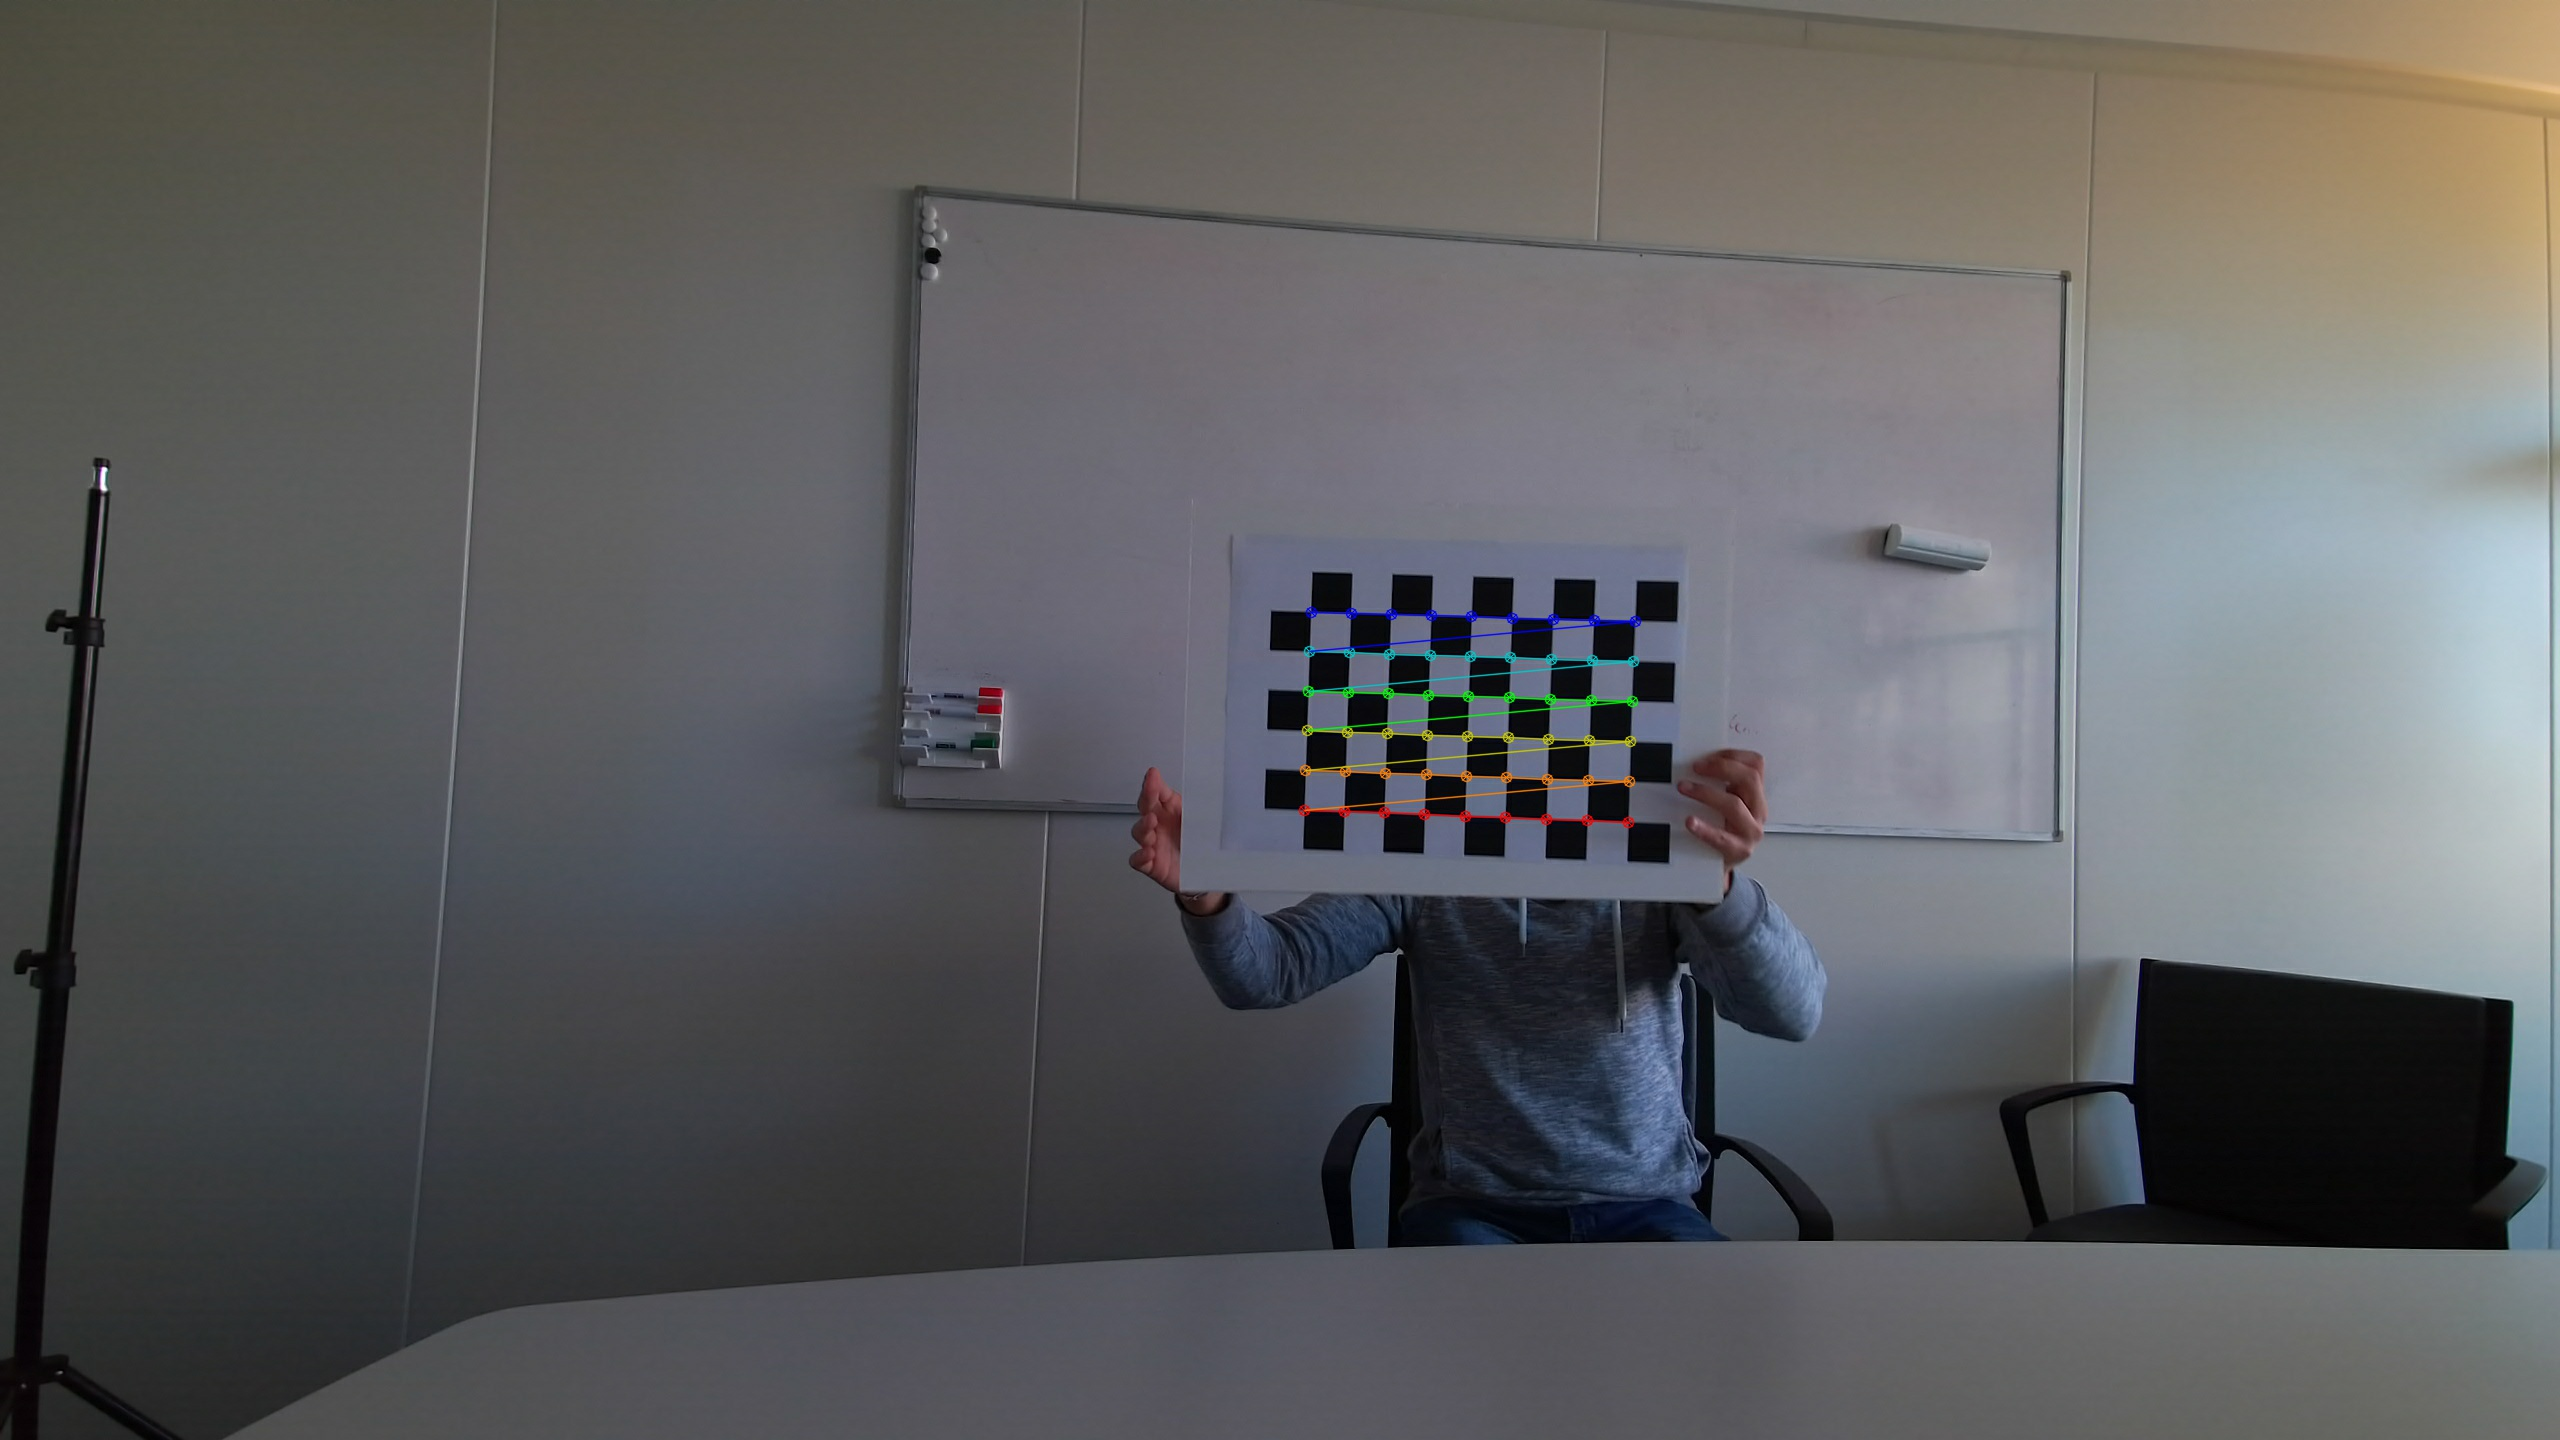
\includegraphics[width=\textwidth]{images/registration/corner_sub_4.jpg}
    \caption{Chessboard viewed from camera 1}
    \label{figure:corner_sub_4}
  \end{subfigure}
  \hfill
  \begin{subfigure}[b]{0.48\textwidth}
    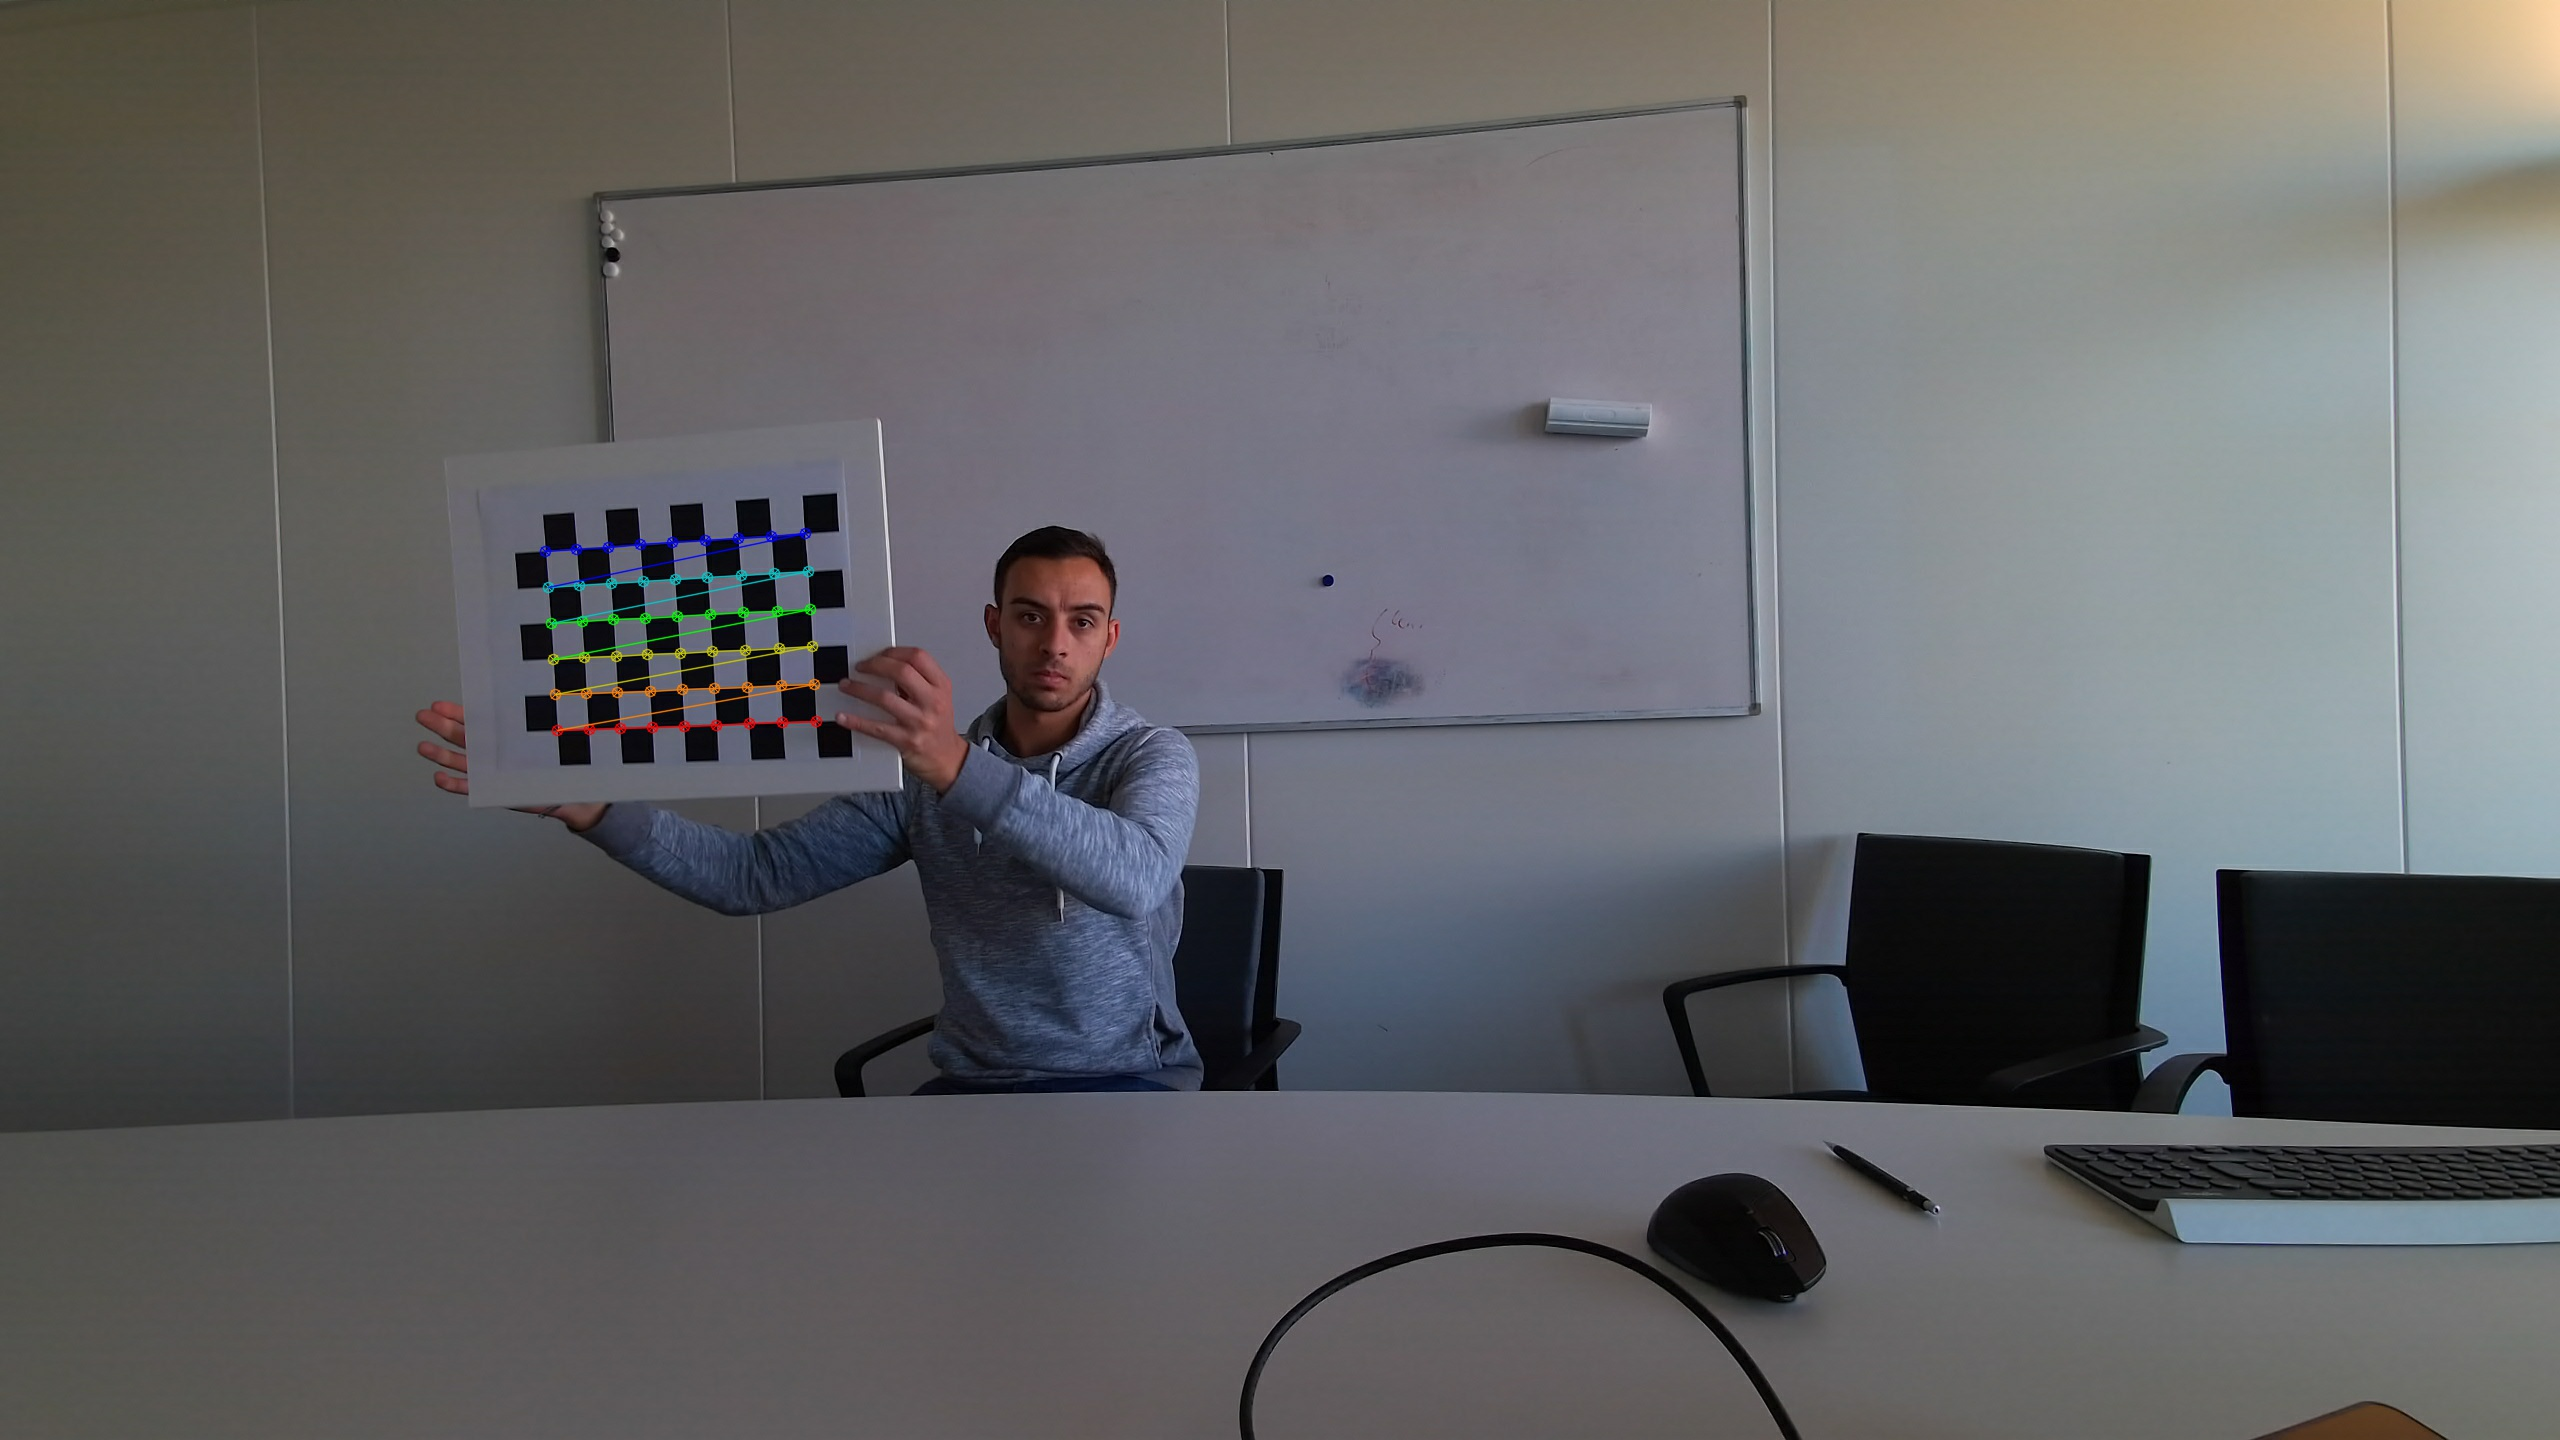
\includegraphics[width=\textwidth]{images/registration/corner_master_4.jpg}
    \caption{Chessboard viewed from camera 2}
    \label{figure:corner_master_4}
  \end{subfigure}
  \caption{Detection of the chessboard corners viewed from both cameras at the same time}
  \label{figure:corner}
\end{figure}

The function \textit{StereoCalibrate} provided by OpenCV is then used. It estimates transformation between two cameras making a stereo pair. One of the outputs is the estimation of the transformation matrix between the coordinate systems of the first and the second cameras.

% \todo{is this figure relevant?}
% \begin{figure}[H]
%     \centering
%     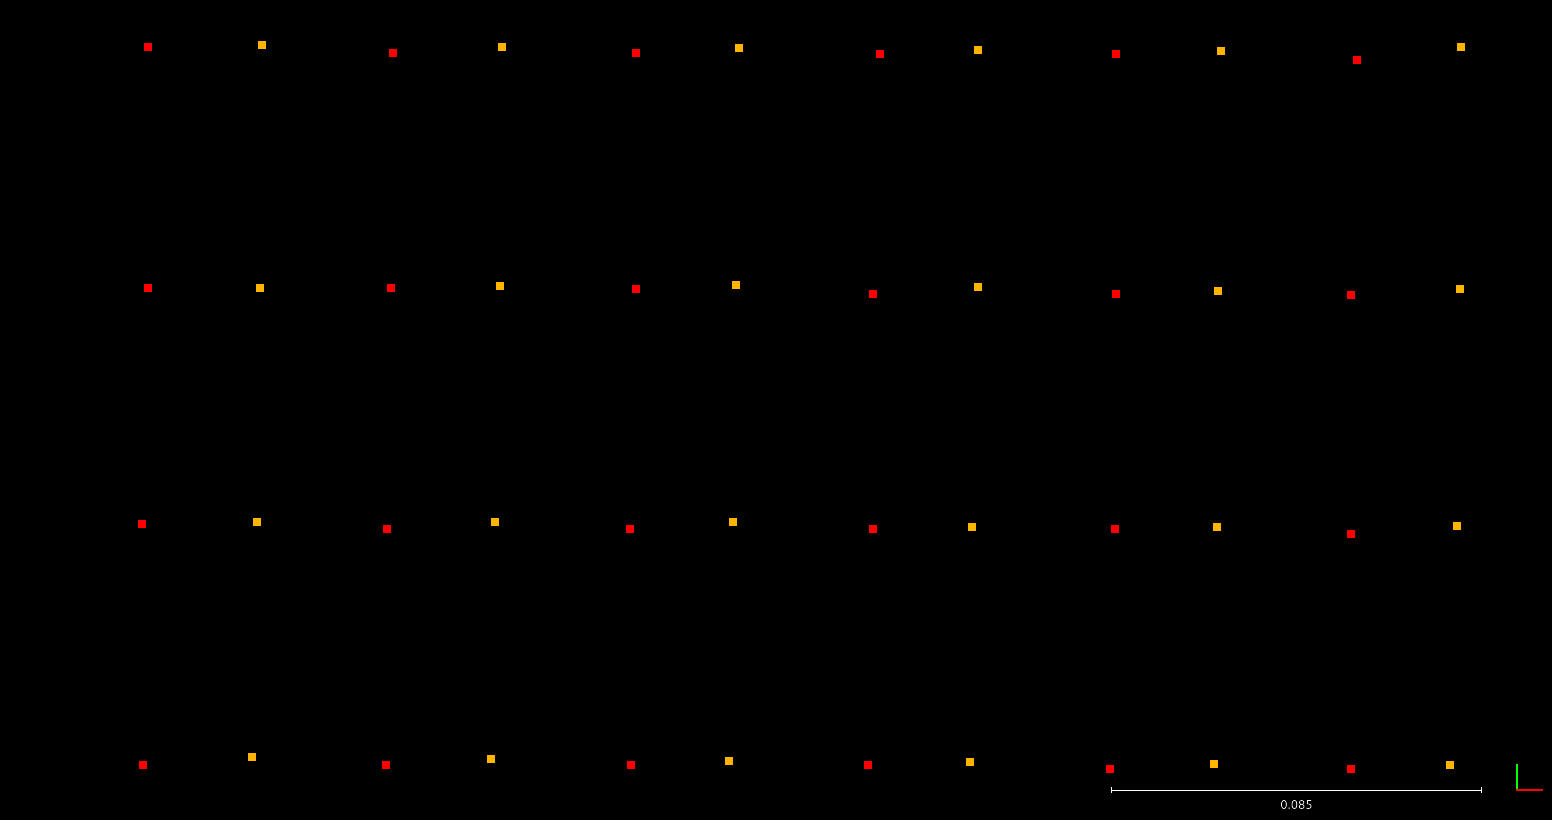
\includegraphics[width=0.65\textwidth]{images/registration/chessboard_transfo.png}
%     \caption{Plan XY. Red points: ChArUco board point cloud from the 1st camera. Yellow points: ChArUco board point cloud from the 2nd camera. Scale is in meter}
%     \label{figure:chessboard_transfo}
% \end{figure}

Table \ref{tab:mae_chessboard} presents the results after applying the found transformation matrix on one of the ChArUco point clouds of figure \ref{figure:pc_arucoboard}. The error in the X-coordinate is quite big, see table \ref{tab:mae_chessboard}. This results in a noticeable misalignment when applied on live sequence with a person in it. Figure \ref{figure:stereo_misaligned} shows a selected frame where the misalignment is visible.

\begin{table}[H]
\centering
\begin{tabular}{c|c|c|c}
 & \textbf{X - coordinate} & \textbf{Y - coordinate} & \textbf{Z - coordinate} \\ \hline
\textbf{Mean Absolute Error {[}mm{]}} & 24.07 & 1.09 & 4.54
\end{tabular}
\caption{Mean absolute error for the stereo calibration experiment with the chessboard}
\label{tab:mae_chessboard}
\end{table}

\begin{figure}[H]
\centering
  \begin{subfigure}[b]{0.48 \textwidth}
    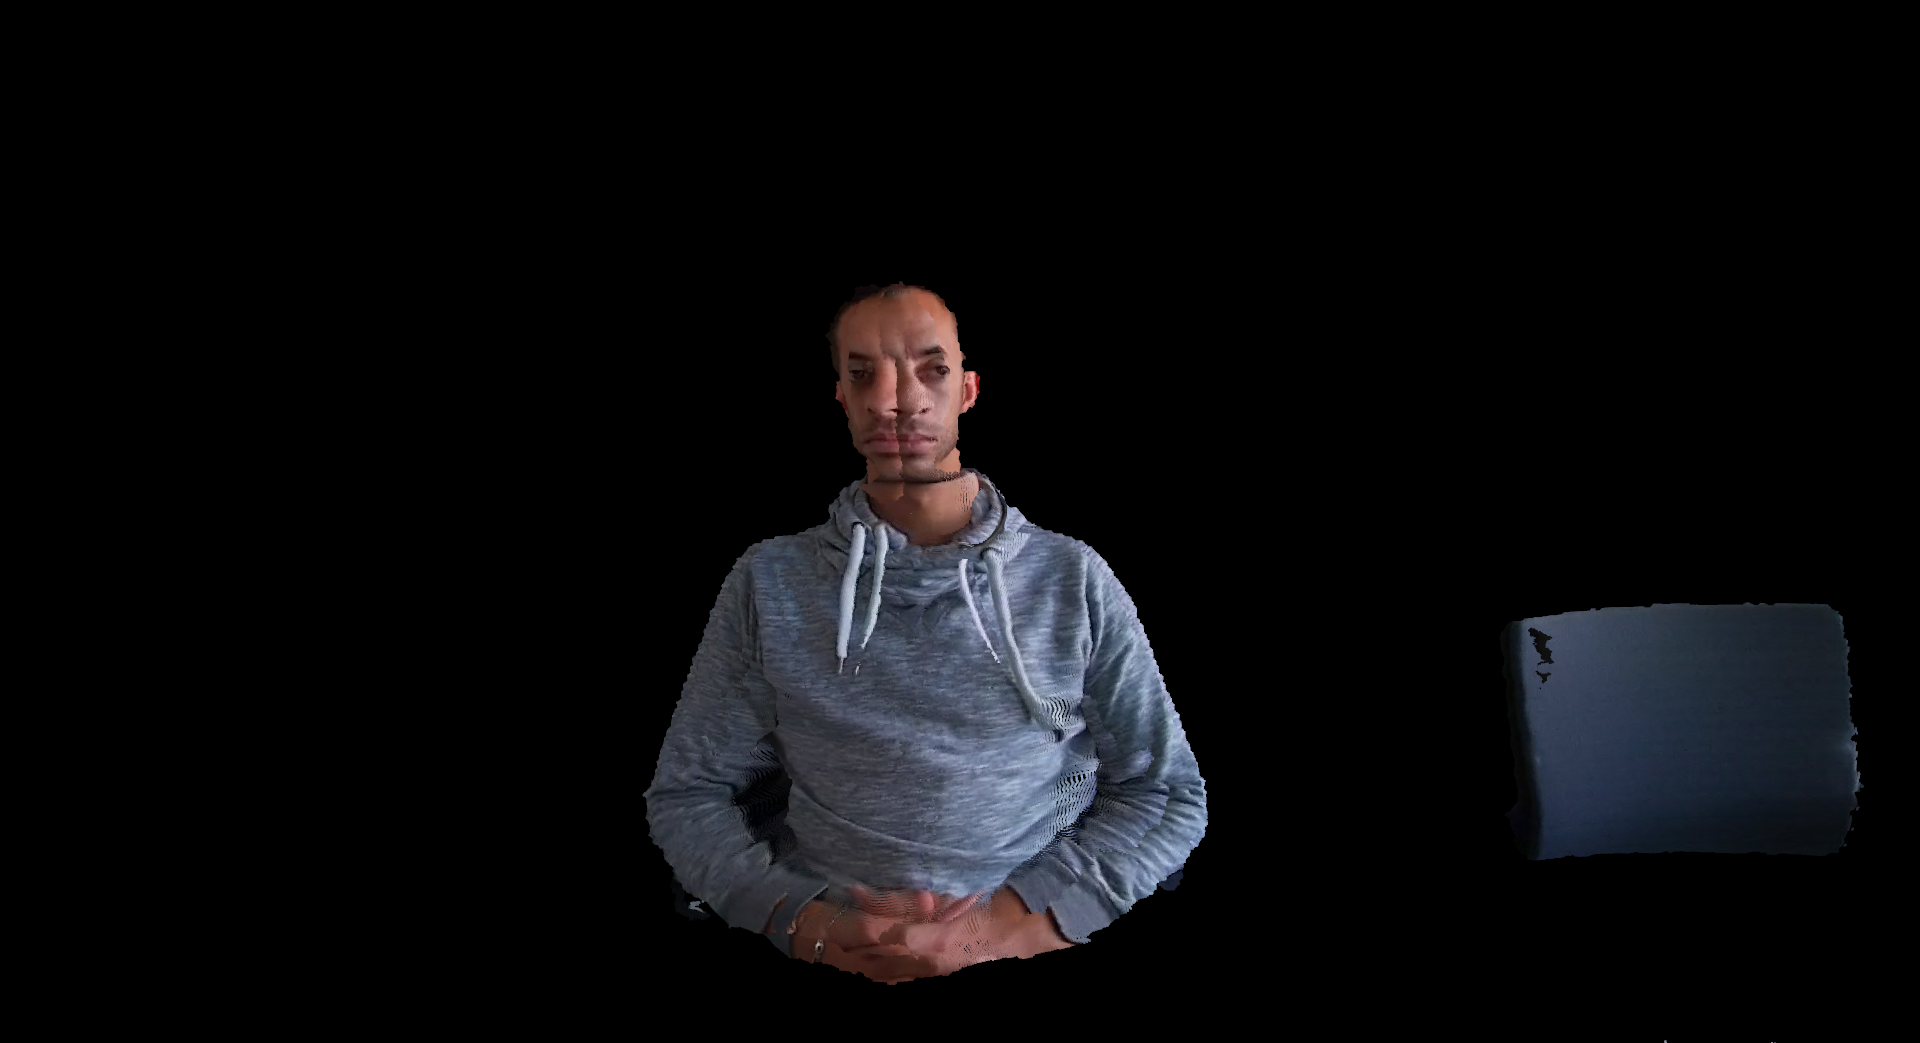
\includegraphics[width=\textwidth]{images/registration/stereo_RGB.png}
    \caption{Alignment after applying the found matrix}
    \label{figure:stereo_RGB}
  \end{subfigure}
  \hfill
  \begin{subfigure}[b]{0.48\textwidth}
    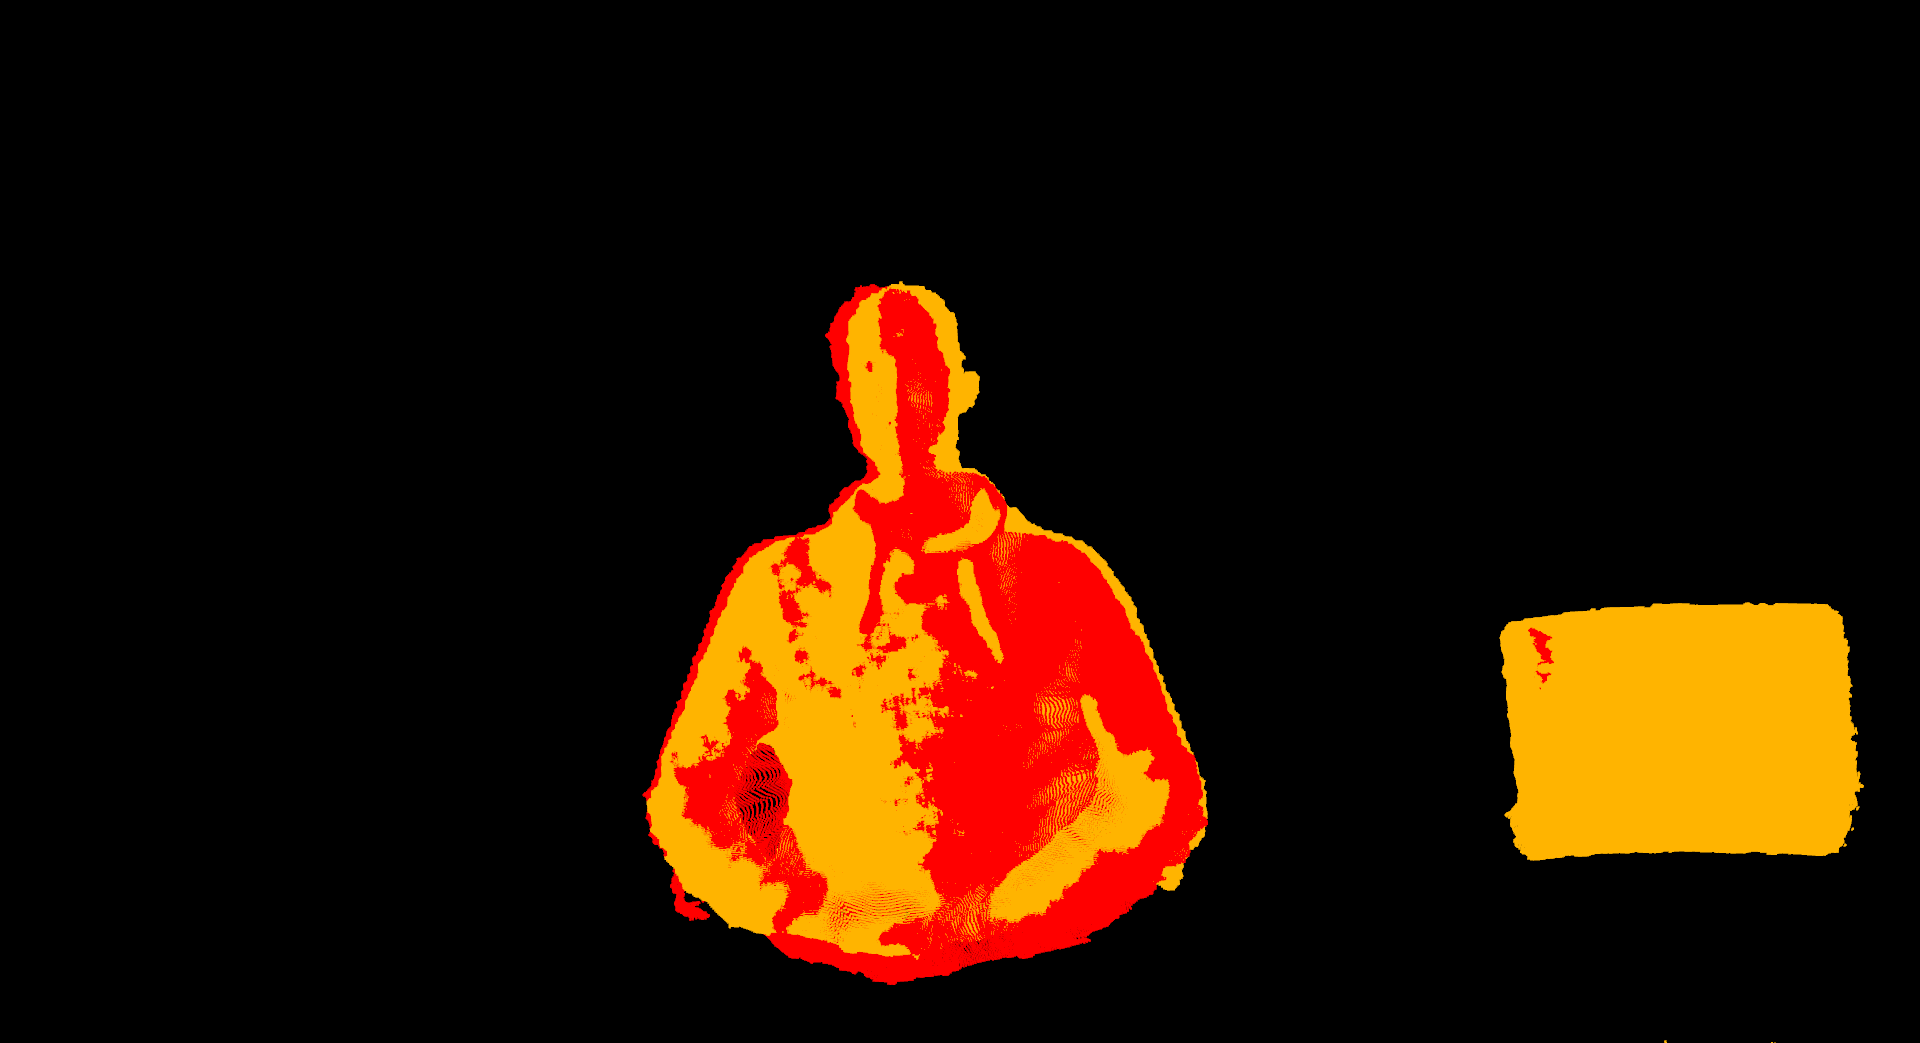
\includegraphics[width=\textwidth]{images/registration/stereo_colored.png}
    \caption{Red: point cloud 1. Yellow: point cloud 2}
    \label{figure:stereo_colored}
  \end{subfigure}
  \caption{Alignment of the two point clouds created from the two different views after applying the transformation matrix found by stereo calibration}
  \label{figure:stereo_misaligned}
\end{figure}

\subsubsection{Proposed method}

The approach explained in section \ref{section:proposed_method} is applied to this experiment. A ChArUco board is placed in the centre of the scene. 100 frames are taken in a synchronised way from both views. The pixel positions of the corners are extracted with their corresponding depth and averaged over the frames. Then two point clouds are created, i.e. one per camera, with the help of equation (\ref{equation:2dTO3d}). Finally, a function provided by Open3D \cite{Zhou2018} is used.

\begin{table}[H]
\begin{tabular}{c|c|c|c}
 & \textbf{X - coordinate} & \textbf{Y - coordinate} & \textbf{Z - coordinate} \\ \hline
\textbf{Mean Absolute Error (MAE) {[}mm{]}} & 0.90 & 0.48 & 0.40
\end{tabular}
\caption{Mean absolute error for the stereo calibration experiment of the proposed method}
\label{tab:mae_proposed_method}
\end{table}

Table \ref{tab:mae_proposed_method} presents the different MAE. As this error is below 1 mm, it is barely visible in a dynamic scene. Figure \ref{figure:proposed_method_alignment} shows a selected frame.

% One can notice the misalignment only when the zoom is quite high, see figure ...

\begin{figure}[H]
\centering
  \begin{subfigure}[b]{0.48 \textwidth}
    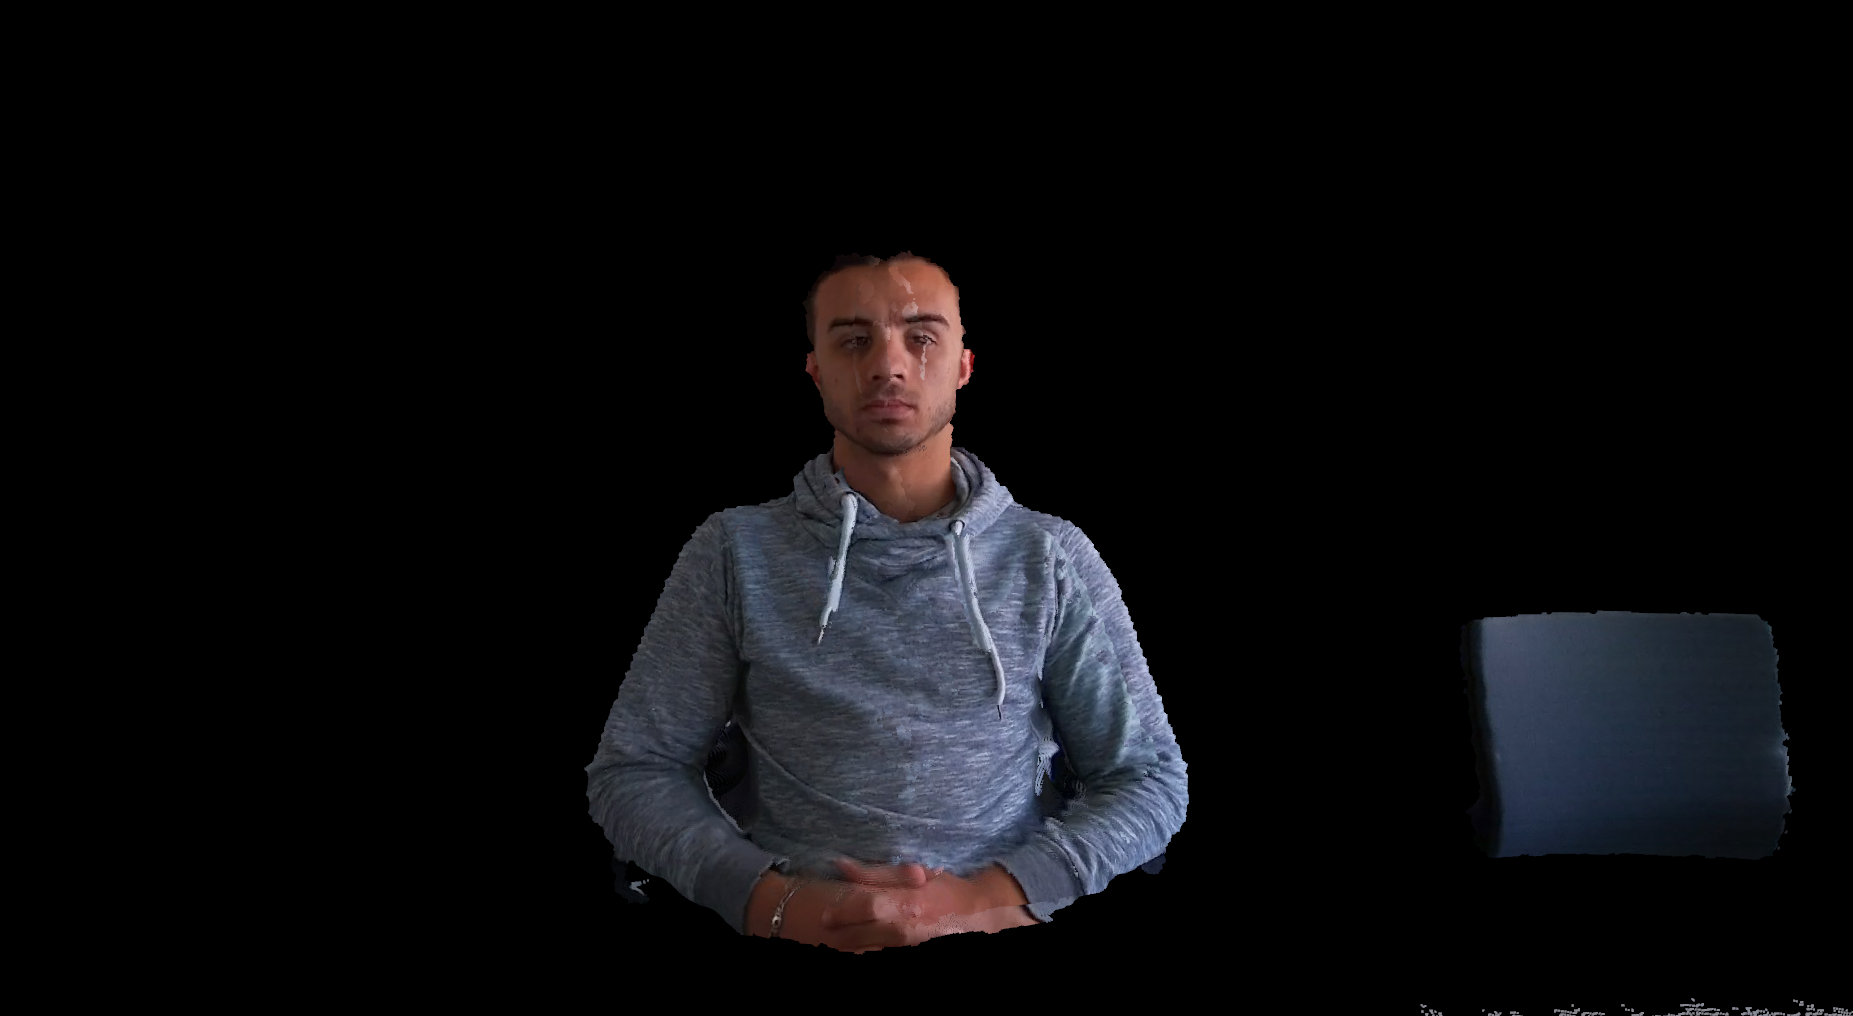
\includegraphics[width=\textwidth]{images/registration/proposed_method_RGB.png}
    \caption{Alignment after applying the found matrix}
    \label{figure:stereo_RGB}
  \end{subfigure}
  \hfill
  \begin{subfigure}[b]{0.48\textwidth}
    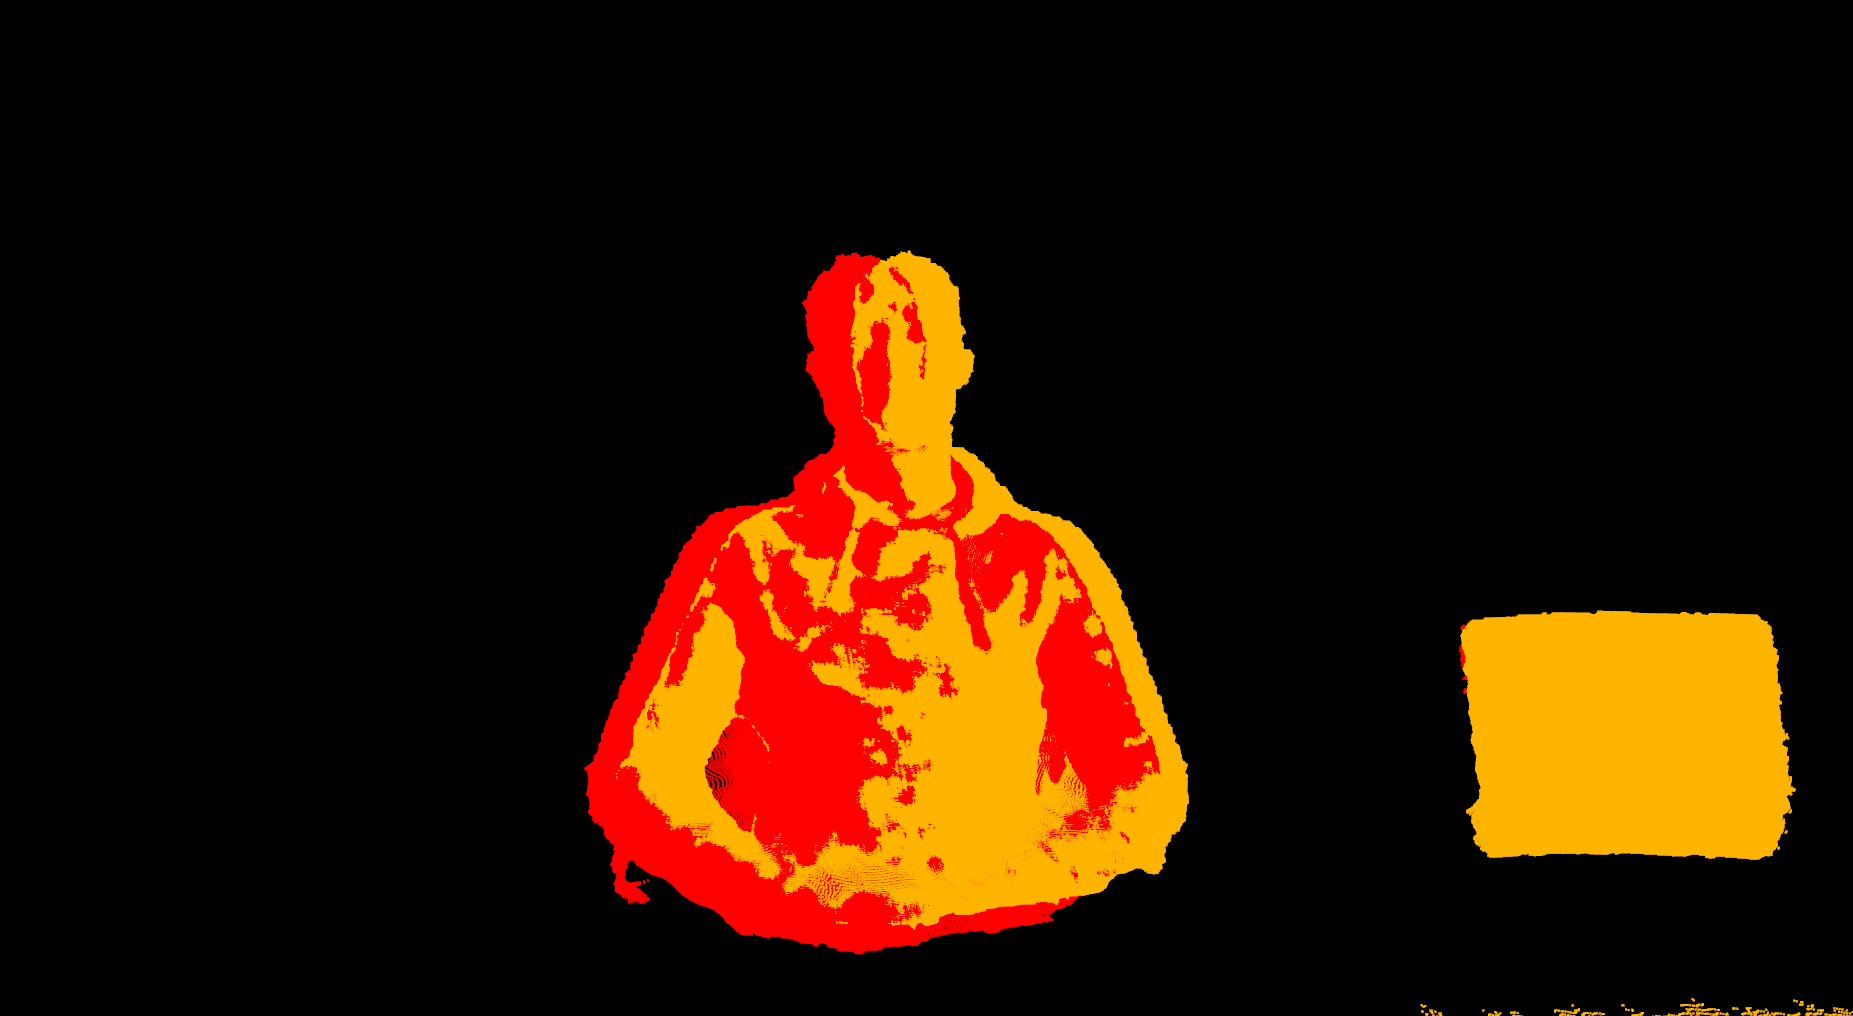
\includegraphics[width=\textwidth]{images/registration/proposed_method_colour.png}
    \caption{Red: point cloud 1. Yellow: point cloud 2}
    \label{figure:stereo_colored}
  \end{subfigure}
  \caption{Alignment of the two point clouds created from the two different views after applying the transformation matrix found by the proposed method}
  \label{figure:proposed_method_alignment}
\end{figure}



Despite a good alignment in the region around the ChArUco board, a small misalignment is visible in the background for example, see figure \ref{figure:proposed_method_background}. One reason could come from the intrinsic parameters. They are used to create the point clouds. So if they are not exact, it could create a slightly deformed point cloud. Another reason  could come from the fact that the background is further away from the board. So even if this error is small on the region around the board, this error becomes more noticeable outside the calibrated region.

\begin{figure}[H]
    \centering
    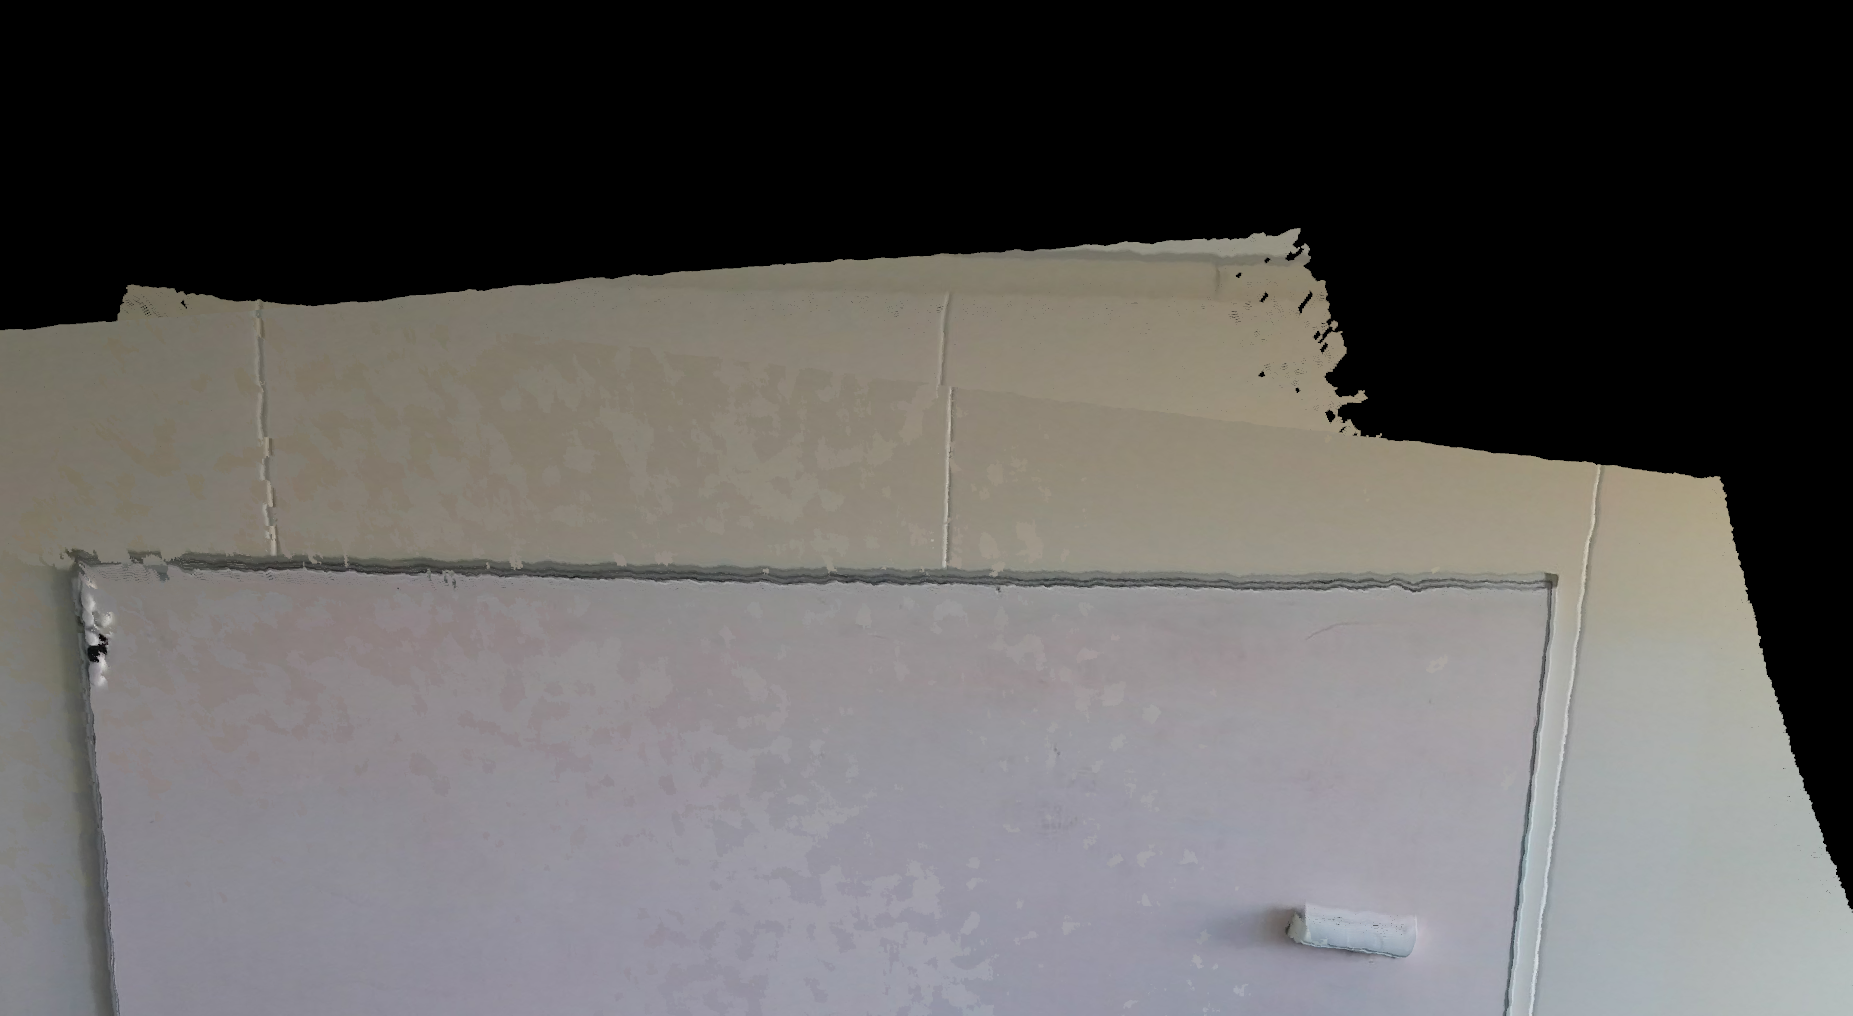
\includegraphics[width=0.65\textwidth]{images/registration/proposed_method_background.png}
    \caption{Small misalignment in the background}
    \label{figure:proposed_method_background}
\end{figure}
